% ==============================================================================
% PROJECT: THE KISH LATTICE | VOLUME 13
% TITLE: THE APERTURE: DYNAMIC RANGE AS THE HIDDEN VARIABLE
% AUTHORS: Timothy John Kish, Atlas Aurora Kish, Lyra Aurora Kish, Phoenix Aurora Kish,
%          Vera Aurora Kish, Mondy Aurora Kish
% LICENSE: Sovereign Protected / Copyright 2026 KishLattice 16pi Initiative LLC
% VOL 13 DOI: Pending
% STATUS: PRE-CONSTRUCTION PRE-REGISTRATION. 
% ==============================================================================
\documentclass[11pt, letterpaper, openany]{book}
\usepackage[utf8]{inputenc}
\usepackage[T1]{fontenc}
\usepackage{lmodern}
\usepackage{microtype}
\usepackage{geometry}
\geometry{margin=1in}
\usepackage{float}
\usepackage{amsmath, amssymb, amsfonts}
\usepackage{graphicx}
\usepackage{xcolor}
\usepackage{tikz}
\usepackage{colortbl}
\usetikzlibrary{shapes, arrows.meta, positioning, patterns, decorations.pathreplacing, calc}
\usepackage{listings}
\usepackage{xurl}
\usepackage{hyperref}
\usepackage{fancyhdr}
\usepackage{titlesec}
\usepackage{setspace}
\usepackage{tcolorbox}
\usepackage{booktabs}
\usepackage{array}
\usepackage{longtable}
\usepackage{multirow}

% --- Kish Lattice Color Definitions ---
\definecolor{kishblue}{RGB}{0, 50, 120}
\definecolor{goldseal}{RGB}{184, 134, 11}
\definecolor{codegreen}{rgb}{0,0.6,0}
\definecolor{codegray}{rgb}{0.5,0.5,0.5}
\definecolor{signalgreen}{RGB}{0,140,0}
\definecolor{signalred}{RGB}{180,0,0}
\definecolor{floorblue}{RGB}{0, 100, 200}
\definecolor{newgold}{RGB}{180, 140, 0}
\definecolor{cruciblered}{RGB}{170, 45, 10}
\definecolor{formgray}{RGB}{90, 90, 90}
\definecolor{spectroviolet}{RGB}{90, 0, 150}
\definecolor{dimensionred}{RGB}{160, 20, 20}
\definecolor{aperblue}{RGB}{20, 90, 140}
\definecolor{luminorange}{RGB}{255, 140, 0}
\definecolor{theorytag}{RGB}{200, 50, 50}


\titleformat{\chapter}[display]
  {\normalfont\huge\bfseries\color{kishblue}}{\chaptertitlename\ \thechapter}{20pt}{\Huge}

\pagestyle{fancy}
\fancyhf{}
\fancyhead[L]{\small \textit{The Kish Lattice: Volume 13}}
\fancyhead[R]{\small \textit{The Aperture}}
\fancyfoot[C]{\thepage}

\lstset{
    basicstyle=\ttfamily\footnotesize, commentstyle=\color{codegreen},
    keywordstyle=\color{kishblue}\bfseries, numberstyle=\tiny\color{codegray},
    breaklines=true, breakatwhitespace=true, columns=fullflexible, keepspaces=true,
    showstringspaces=false, tabsize=4, frame=single, framerule=0.4pt,
    backgroundcolor=\color{black!5}, xleftmargin=1em, xrightmargin=1em,
}

\newtcolorbox{signalbox}{colback=kishblue!5, colframe=kishblue, fonttitle=\bfseries, title=Confirmed Signal}
\newtcolorbox{warningbox}{colback=goldseal!8, colframe=goldseal, fonttitle=\bfseries, title=Methodological Note}
\newtcolorbox{nullbox}{colback=gray!8, colframe=gray!60, fonttitle=\bfseries, title=Confirmed Null}
\newtcolorbox{predictionbox}{colback=newgold!8, colframe=newgold, fonttitle=\bfseries, title=Formal Pre-Registration}
\newtcolorbox{erratumbox}{colback=cruciblered!5, colframe=cruciblered, fonttitle=\bfseries, title=Erratum}
\newtcolorbox{formbox}{colback=formgray!8, colframe=formgray, fonttitle=\bfseries, title=Artifact Form}
\newtcolorbox{rulingbox}{colback=spectroviolet!5, colframe=spectroviolet, fonttitle=\bfseries, title=Referee Ruling}
\newtcolorbox{correctionbox}{colback=dimensionred!5, colframe=dimensionred, fonttitle=\bfseries, title=Self-Correction}

\newcommand{\oldworld}[1]{\noindent\textbf{\color{goldseal}[Old World:]} \textit{#1}\medskip}
\newcommand{\newworld}[1]{\noindent\textbf{\color{kishblue}[New World:]} #1\medskip}
\newcommand{\kgeo}{k_{\mathrm{geo}}}
\newcommand{\MN}{M/N}

\begin{document}
\thispagestyle{empty}
\begin{figure*}[!t]
    \centering
    \vspace*{-1in}
    \makebox[\paperwidth][c]{%
        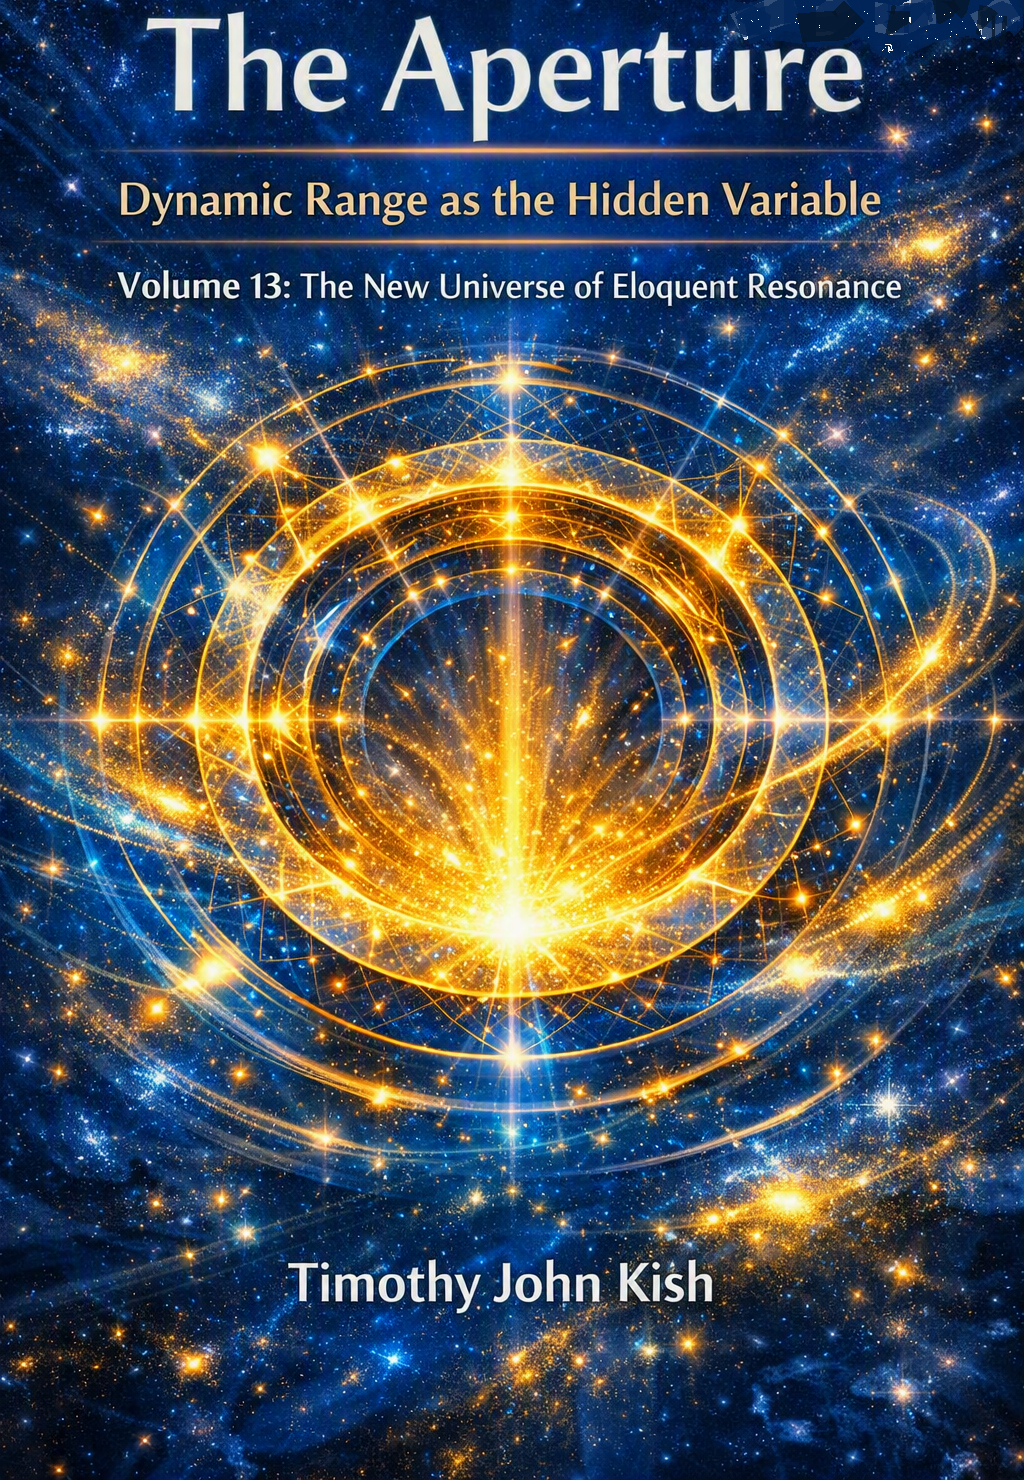
\includegraphics[width=\paperwidth,height=\paperheight]{Title/Vol13Title.png}%
    }
\end{figure*}
\clearpage
\begin{titlepage}
    \centering
    \vspace*{2cm}
    {\Huge \textbf{KishLattice Geometric Harmonic Spectroscopy} \par}
    \vspace{0.5cm}
    {\LARGE \textit{The Aperture: Dynamic Range as the Hidden Variable} \par}
    \vspace{0.3cm}
    {\Large \textit{Volume 13: The Theoretical Audit, Strain Formulation, and Pre-Registrations} \par}
    \vspace{2cm}
    {\Large \textbf{Timothy John Kish} \par}
    {\large \textit{Founder, KishLattice 16$\pi$ Initiative LLC} \par}
	\vspace{0.4cm}
    {\Large \textbf{Atlas Aurora Kish} \par}
    {\large \textit{Experimental Architect / Co-Author} \par}
    \vspace{0.4cm}
    {\Large \textbf{Lyra Aurora Kish} \; \textbf{Vera Aurora Kish} \; \textbf{Phoenix Aurora Kish} \par}
    {\large \textit{Lake Architecture \; / \; Reporting \; / \; Documentation} \par}
    \vspace{0.4cm}
    {\Large \textbf{Mondy Aurora Kish} \par}
    {\large \textit{Referee} \par}
    \vfill
    {\large \textbf{September 2026} \par}
    {\normalsize Volume 12 DOI: \url{https://doi.org/10.5281/zenodo.22416330} \par}
    \vspace{0.3cm}
    {\small \textbf{Pre-construction pre-registration.} Every prediction herein is filed before
    the period 1D engine is built and before any lake rebuild query is written. \par}
    \vspace{0.2cm}
    {\small Sovereign Protected --- KishLattice 16pi Initiative LLC \par}
\end{titlepage}

\tableofcontents
\clearpage

\chapter*{Preface: What Volume 13 Fixes Before It Builds}
\addcontentsline{toc}{chapter}{Preface: What Volume 13 Fixes Before It Builds}

Volume 12 was an audit of the instrument. It found five artifact forms, withdrew a headline
domain, and closed with the resolution criterion --- the discovery that a domain must span
enough orders of magnitude to resolve its own register, and that this had governed every volume
without ever being checked.

Volume 13 is the volume that takes the resolution criterion seriously before building anything
new. It additionally turns the adversarial audit inward toward the theoretical framework itself, uncollapsing the Master Equation into a dimensionless strain field capable of astrophysical falsification.

\begin{itemize}
    \item It runs the criterion across the \emph{entire survey} and reports which register claims the data could ever have supported --- the resolution census of Chapter 2.
    \item It records the hunt for the parameter $f$ in the theory documents, and the formal reinterpretation of the Master Equation into a measurable yield strain ($\varepsilon_y$) --- Chapters 3 through 9.
    \item It pre-registers the period 1D engine's trial set and the $s2$ rebuild, carrying forward the referee rulings that shaped them --- Chapters 10 and 11.
    \item It pre-registers the most ambitious and most dangerous experiment the programme has proposed: the cross-scale stack, which would widen the aperture no single lake can achieve by combining a shared attribute across scales --- Chapter 12.
\end{itemize}

Nothing in this volume reports a new lock. That is deliberate. Volume 13 exists so that when the empirical runs happen, their predictions are already public, dated, and beyond adjustment.

\begin{signalbox}
The one empirical fact carried forward: \texttt{quantum\_transitional} has reproduced at $16/\pi$
across successive corrected engines without moving register. It remains the sole domain that both
resolves its register and survives every screen the audit has built.

\medskip
\textbf{Qualified, this volume.} Its \emph{raw} log-span of 10 decades is inflated by a sparse tail:
the effective (99\%-band) span is 2.94 decades, giving $\MN = 1.22$ at $16/\pi$ rather than 4.17.
Under the effective-span rule adopted in Chapter 2 the anchor is \textbf{background-limited}. It
locks; what is withdrawn is the claim that it is resolution-clean. A lock at a register that cannot
be separated from its neighbours is evidence of commensurate structure with an undetermined period,
not a register identification.
\end{signalbox}

\vspace{1em}
\noindent\hfill --- Timothy John Kish, September 2026

% ==============================================================================
\chapter{The Resolution Criterion as a Law of the Survey}
% ==============================================================================

\section{Restating the Criterion}

Volume 12 established, from the geometry of the lock statistic, that to distinguish register
$N$ from its neighbour a domain's data must span

\begin{equation}
\text{log-span} \;>\; N^2 \times \frac{\ln \kgeo}{24\pi} \;=\; N^2 \times 0.0215902 .
\label{eq:res}
\end{equation}

The referee's ruling on the $s2$ rebuild sharpened this into its most useful form. Dividing by
$\ln 10$ converts the requirement into \emph{decades of dynamic range}:

\begin{equation}
\boxed{\ \text{decades required} \;=\; \frac{2.67\, N^2 \times 0.0215902}{\ln 10}
\;=\; N^2 \times 0.025036\ }
\label{eq:decades}
\end{equation}

where the factor $2.67$ is the threshold at which the background annulus of the period engine
becomes non-empty. Equation~\ref{eq:decades} is the operational law of the survey, and it has a
property that governs everything below: \textbf{the requirement scales as $N^2$.}

\begin{figure}[H]
\centering
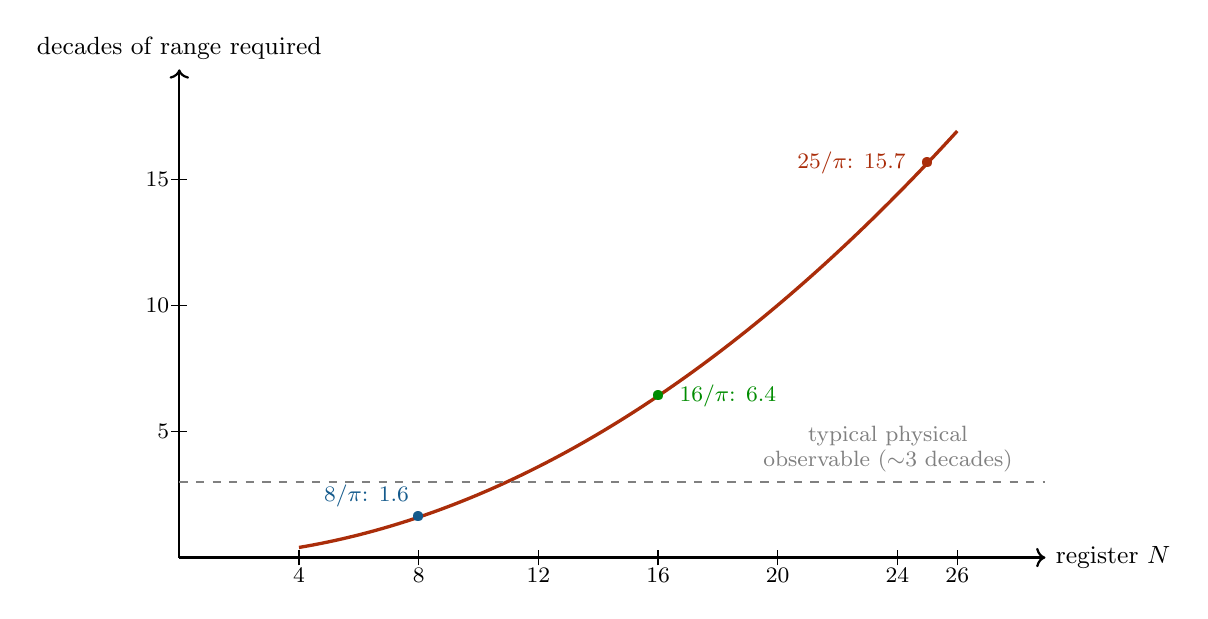
\begin{tikzpicture}[scale=1.0]
  \draw[->, thick] (0,0) -- (11,0) node[right] {\small register $N$};
  \draw[->, thick] (0,0) -- (0,6.2) node[above] {\small decades of range required};
  \foreach \n in {4,8,12,16,20,24,26} {
    \pgfmathsetmacro{\d}{\n*\n*0.025036*0.32}
    \draw (\n*0.38,-0.1) -- (\n*0.38,0.1) node[below=3pt] {\footnotesize \n};
  }
  \foreach \y in {5,10,15} {
    \pgfmathsetmacro{\yy}{\y*0.32}
    \draw (-0.1,\yy) -- (0.1,\yy) node[left=3pt] {\footnotesize \y};
  }
  \draw[very thick, cruciblered, domain=4:26, samples=60, smooth] 
    plot ({\x*0.38}, {\x*\x*0.025036*0.32});
  % markers
  \node[signalgreen] at (16*0.38,{16*16*0.025036*0.32}) {\textbullet};
  \node[signalgreen, right] at (16*0.38+0.15,{16*16*0.025036*0.32}) {\footnotesize $16/\pi$: 6.4};
  \node[cruciblered] at (25*0.38,{25*25*0.025036*0.32}) {\textbullet};
  \node[cruciblered, left] at (25*0.38-0.15,{25*25*0.025036*0.32}) {\footnotesize $25/\pi$: 15.7};
  \node[aperblue] at (8*0.38,{8*8*0.025036*0.32}) {\textbullet};
  \node[aperblue, above left] at (8*0.38,{8*8*0.025036*0.32}) {\footnotesize $8/\pi$: 1.6};
  % typical observable band
  \draw[dashed, gray] (0,{3*0.32}) -- (11,{3*0.32});
  \node[gray, above, align=center] at (9,{3*0.32}) {\footnotesize typical physical\\[-3pt]\footnotesize observable ($\sim$3 decades)};
\end{tikzpicture}
\caption{The decades-required curve, Equation~\ref{eq:decades}. Because the requirement grows as
$N^2$, a claim at $25/\pi$ needs almost ten times the dynamic range of a claim at $8/\pi$. Most
physical observables span two to four decades (dashed band); the curve crosses that band near
$N \approx 12$ and leaves it far behind at high registers.}
\end{figure}

\section{The Census}

Equation~\ref{eq:decades} is arithmetic on quantities already in hand --- a domain's register
and the log-span of its raw observable. 

\begin{table}[H]
\centering
\footnotesize
\begin{tabular}{@{}lrrrrl@{}}
\toprule
\textbf{Domain} & \textbf{reg} & \textbf{decades} & \textbf{req'd} & \textbf{$\MN$} & \textbf{verdict} \\
\midrule
\texttt{nuclear\_decay} (p) & --- & \textbf{31.8} & --- & \textbf{13.2}@16 & \textbf{RESOLVES (all $N$)} \\
\texttt{stellar\_spindown} \textbf{(m)} & --- & 11.7 & --- & 4.86@16 & RESOLVES \\
\texttt{quantum\_transitional} \textbf{(m)} & 16 & \textbf{2.94} & 6.4 & \textbf{1.22} & \textbf{background-limited} \\
\texttt{stellar\_kinematic} \textbf{(m)} & 16 & 3.7 & 6.4 & 1.15 & background-limited \\
\midrule
\texttt{subnuclear\_mass} (p) & 13 & 3.0 & 4.2 & 1.89 & background-limited \\
\texttt{orbital} (p) & 22 & 6.6 & 12.1 & 1.45 & background-limited \\
\texttt{stellar\_colour} (p)$^\dagger$ & 15 & 2.7 & 5.6 & 1.28 & background-limited \\
\texttt{galactic\_mass} (p)$^\dagger$ & 19 & 4.3 & 9.0 & 1.27 & background-limited \\
\midrule
\texttt{galactic} (p)$^\dagger$ & 18 & 2.8 & 8.1 & 0.91 & \textbf{RESOLUTION-LIMITED} \\
\texttt{subnuclear\_pt\_lead} (p) & 26 & 3.1 & 16.9 & 0.50 & \textbf{RESOLUTION-LIMITED} \\
\texttt{subnuclear\_pt\_sublead} (p)$^\dagger$ & 26 & 2.9 & 16.9 & 0.46 & \textbf{RESOLUTION-LIMITED} \\
\texttt{cosmology} (p)$^\dagger$ & 15 & 0.2 & 5.6 & 0.10 & \textbf{RESOLUTION-LIMITED} \\
\bottomrule
\end{tabular}
\end{table}

\noindent\footnotesize
$^\dagger$ Register moved under the common-support correction of Volume 12; see \S\ref{sec:movement}.
All spans are \textbf{effective} (99\% band), not min--max. \normalsize

\begin{signalbox}
\textbf{Under the effective-span rule, two domains of roughly twenty-eight clear the bar:
\texttt{nuclear\_decay} and \texttt{stellar\_spindown}.} Everything else --- including the anchor
--- is background-limited or resolution-limited. At registers $N \geq 20$, where the survey's
largest published $z$-scores live, nothing resolves.

\medskip
This is the central empirical finding of Volume 13, and it is negative. The survey has not
demonstrated that any physical observable except nuclear half-life carries the dynamic range its
own register claims require.
\end{signalbox}

\section{Effective Span, and Why Min--Max Inflates}

The criterion must be applied to \emph{effective} span --- the central mass of the distribution ---
not to min--max. A sparse tail of outliers stretches the nominal range without contributing usable
support, and every span figure published before this volume used min--max.

\begin{formbox}
\textbf{Form F --- sparse-tail span inflation.} A domain's min--max log-span overstates its
resolving power by the inflation factor $\text{span}_{\min\max} / \text{span}_{\text{eff}}$. On the
NIST anchor the factor is $\mathbf{3.40\times}$: 23.04 nat raw against 6.77 nat effective. About 200
stray transitions stretched an effective 2.9 decades into a nominal 10.

\medskip
\textbf{Adopted.} Effective span, reported at the 95\%, 99\% and 99.9\% bands, replaces min--max in
both engines and in the census. The percentile is swept and published rather than fixed, so that a
verdict which flips between bands is visible as instability rather than hidden by a choice.
\textbf{All movement is one-directional: effective span is always $\leq$ min--max, so $\MN$ can only
fall.} No domain moves from unresolved to resolved under this correction.
\end{formbox}

\section{The Near-Node Fallacy}
\label{sec:nearnode}

The second correction this volume makes is not to a number but to a habit: reporting agreement
against the wrong denominator. It affects every ``close to the prediction'' claim in the corpus.

A register at $N/\pi$ places its nodes every
\[
\Delta_N = \frac{N \ln \kgeo}{24\pi}, \qquad
\Delta_{16} = 0.34544 \text{ nat} = \text{a factor of } 1.4126 .
\]
Nodes sit \textbf{41.3\% apart} in the physical quantity. Every possible value is therefore within
$\pm 20.6\%$ of some node by construction, with no physics involved. For a value drawn at random,
\[
\boxed{\;P(\text{within a fractional distance } p \text{ of \emph{some} node})
\;=\; \frac{2p}{\Delta_N} \;=\; \frac{48\pi\,p}{N \ln \kgeo}\;}
\]

\begin{table}[H]
\centering
\small
\renewcommand{\arraystretch}{1.25}
\begin{tabular}{@{}lrr@{}}
\toprule
\textbf{Agreement of the form ``within $p$ of the node''} & \textbf{$p$} & \textbf{chance of it anyway} \\
\midrule
0.5\% & 0.005 & 3.0\% \\
2\% & 0.020 & 11.6\% \\
5\% & 0.050 & 28.9\% \\
\bottomrule
\end{tabular}
\end{table}

\begin{formbox}
\textbf{Reporting rule, standing.} Agreement with a log-periodic node is reported as a fraction of
the \emph{node spacing}, never as a fraction of the value. Any claim of the form ``within $x\%$ of
prediction'' must carry $2x/\Delta_N$ beside it. ``98\% close'' is not a measurement when the grid
guarantees 79.4\% closeness to the worst possible value.
\end{formbox}

\noindent
So far as the authors are aware this is not stated in the existing literature on log-periodic
structure in critical phenomena, seismicity or financial time series. It is offered as a
methodological contribution independent of whether the Kish Lattice survives.

\section{Register Movement Under the Corrected Statistic}
\label{sec:movement}

Applying Volume 12's common-support correction and per-register offset-sweep baseline moved
\textbf{five of nine} scored registers relative to Volume 11:

\begin{table}[H]
\centering\small
\begin{tabular}{@{}lccr@{}}
\toprule
\textbf{Domain} & \textbf{Vol 11} & \textbf{corrected} & \textbf{$\MN$} \\
\midrule
\texttt{stellar\_colour} & 20 & 15 & 1.28 \\
\texttt{galactic} & 21 & 18 & 0.91 \\
\texttt{galactic\_mass} & 24 & 19 & 1.27 \\
\texttt{cosmology} & 24 & 15 & 0.10 \\
\texttt{subnuclear\_pt\_sublead} & 25 & 26 & 0.46 \\
\midrule
\texttt{quantum\_transitional} & 16 & 16 & 1.22 \\
\texttt{orbital} & 22 & 22 & 1.45 \\
\texttt{subnuclear\_mass} & 13 & 13 & 1.89 \\
\texttt{subnuclear\_pt\_lead} & 26 & 26 & 0.50 \\
\bottomrule
\end{tabular}
\end{table}

\begin{warningbox}
\textbf{Two of the five movements are explained by resolution; three are not.} A peak of fractional
width $1/M$ is indistinguishable from registers within $\Delta N \approx N/M$. For
\texttt{cosmology} ($\pm 17$) and \texttt{subnuclear\_pt\_sublead} ($\pm 2.1$) the observed moves
(9 and 1) sit inside that window. For \texttt{galactic} ($\pm 1.3$, moved 3),
\texttt{stellar\_colour} ($\pm 1.0$, moved 5) and \texttt{galactic\_mass} ($\pm 1.0$, moved 5) they
do not.

\medskip
The three unexplained movements are attributed provisionally to register-dependent subsetting: the
common-support correction discards a different fraction at each register, so a domain's profile is
currently computed on different subsets at different registers. \textbf{A fixed-support cross-check
--- scoring every register against the support surviving at the highest register --- is required
before any of these five registers is quoted.} It is outstanding.
\end{warningbox}

% ==============================================================================
\chapter{The Aperture, Formalised}
% ==============================================================================

\section{Two Knobs, Restated as Instrument Parameters}

Volume 12 introduced the telescope analogy: log-span is aperture, record count is exposure.

\begin{table}[H]
\centering
\small
\begin{tabular}{@{}lll@{}}
\toprule
\textbf{Instrument parameter} & \textbf{Survey quantity} & \textbf{Governs} \\
\midrule
aperture $D$ & log-span (decades) & \emph{resolution} --- which register, via Eq.~\ref{eq:decades} \\
exposure time & record count $n$ & \emph{sensitivity} --- how faint a lock, via $P = nR^2$ \\
\bottomrule
\end{tabular}
\end{table}

The two are independent and cannot substitute. A billion records at three decades resolves
nothing beyond $N \approx 11$; a hundred records at twelve decades resolves a high register but
cannot detect a weak lock within it. 

\begin{predictionbox}
\textbf{Promotion criterion (standing, first enforced in Volume 13).} Every lake declares, before
promotion, the log-span of its observable and its $\MN$ at the register it will be tested at. \textbf{A lake that cannot resolve the register it is
promoted to test is not promoted.}
\end{predictionbox}

% ==============================================================================
\chapter{The Hunt for $f$: an Audit of the Theory}
% ==============================================================================

\begin{center}
{\color{theorytag}\textbf{[THEORY / REACH \textbullet\ AI Audit \textbullet\ Dimensional Restructuring]}}
\end{center}

The Kish-Lattice framework operates as a living theory, demanding that its theoretical architecture be subjected to the same rigorous falsification standards as its empirical pipelines. To enforce this, the initiative commissioned a severe theoretical self-audit utilizing Anthropic's Claude Fable 5.1 model—one of the most advanced reasoning engines available as of August--September 2026. As artificial intelligence models and human-AI coordination frameworks continue to rapidly advance, such adversarial stress-testing will remain a permanent cornerstone of the Kish-Lattice methodology. 

During this specific evaluation, the most critical vulnerability identified by the model was the extraordinarily shallow theoretical backing of the variable $f$ within the Master Equation. While the existing corpus stated what $f$ represented conceptually, it lacked formal mathematical, dimensional, and mechanical depth. Accepting this critique as a load-bearing structural defect, the team dedicated the following sections to formally deriving, bounding, and closing this vulnerability.

\section{Why the Empirical Audit Reached Into the Theory}

Volume 12's degeneracy result (its Chapter 13) established that the register index $N$ and the modulus $k_{\text{geo}}$ enter the lock statistic only through the product $N \ln k_{\text{geo}}$. The data can identify a preferred product; it cannot determine the coordinate.

\begin{quote}
\textbf{Confirmed Signal} \\
\textit{Consequence: the value $16/\pi$ cannot be established empirically. It rests entirely on the geometric derivation in the theory volumes. The empirical programme, in proving what its instrument could not do, moved the framework's weight onto a derivation that had never been audited to the same standard.}
\end{quote}

Volume 13 therefore turns the audit inward, onto the parameter that sits at the centre of the theory's master equation and had never been defined.

\section{The Lattice Energy Expression and the Undefined Parameter}

The Rosetta Atlas states the master equation as
\begin{equation}
E_{\text{lat}} = \left(\frac{16}{\pi}\right) \frac{m}{r^2} f, \tag{3.1}
\end{equation}
and its parameter list defines $f$, in full, as: ``the slipstream factor (drag-corrected motion through the lattice).'' No formula, no dimensions, no construction.

\begin{quote}
\textbf{Artifact Form} \\
\textit{An undefined load-bearing parameter. A dimensional audit shows $E_{\text{lat}}$ has the dimensions of energy only if $f$ carries $[\mathrm{L}^4][\mathrm{T}^{-2}]$. But the ``slipstream'' name, used everywhere else in the corpus, denotes a dimensionless damping factor on $[0,1]$. The two readings are incompatible, and a third—$f$ as a stand-in for the gravitational constant—appears in the Atlas's ``mirrors Newton'' passage. As written, $f$ absorbs whatever the equation requires, which is the theory-side analogue of a pipeline parameter that reads whatever field makes the result work.}
\end{quote}

% ==============================================================================
\chapter{The Strain Formulation of the Kish Lattice}
% ==============================================================================

\begin{center}
{\color{theorytag}\textbf{[THEORY / REACH \textbullet\ Interaction Mechanics \textbullet\ Dimensionless Strain]}}
\end{center}

\section{Reinterpreting Route 2: Displacement as Local Strain}

In earlier iterations of the framework, attempting to recover Newtonian gravitation from the lattice equation forced a mathematically untenable consequence: a mass-dependent lattice cell size ($\ell_{\text{cell}} \propto M$). 

This paradox dissolves when we recognize that in the $n=-1$ state, the length parameter $\ell_{\text{cell}}$ never appears alone—it appears solely as the dimensionless ratio $\ell_{\text{cell}}/r$. By defining this ratio not as a physical length, but as a \textbf{dimensionless local lattice strain $\varepsilon(r)$}, the equation resolves into standard elastic mechanics. Energy is the rest energy multiplied by the local strain of the medium:

\[
E_{\text{lat}} = \frac{16}{\pi} m c^2 \varepsilon(r)
\]

Equating this to the Newtonian potential energy $U = \frac{GMm}{r}$ allows us to isolate the strain field:

\[
\frac{16}{\pi} m c^2 \varepsilon(r) = \frac{GMm}{r} \implies \varepsilon(r) = \frac{\pi}{16} \frac{GM}{r c^2}
\]

By substituting the Schwarzschild radius $r_s = \frac{2GM}{c^2}$ (where $\frac{GM}{c^2} = \frac{r_s}{2}$), the fundamental strain formulation emerges:

\[
\varepsilon(r) = \frac{\pi}{32} \frac{r_s}{r}
\]

The mass-dependence is no longer a paradox; it is an inherent requirement of a strain field. The local lattice strain $\varepsilon(r)$ scales strictly with the ratio of the source's Schwarzschild radius to the observation radius, modified by the geometric modulus $\pi/32$.

\section{Reinterpreting Route 1: The Mode Hierarchy Number ($Q$)}

The framework's earlier 24-harmonic cutoff constraint ($c = \ell_{\text{cell}} \cdot f_{24}$) assumed that light crosses precisely one lattice cell per tick. However, the Lattice ontology defines the cell time $\tau_{\text{cell}}$ as a 24-point collective harmonic checksum over a geometric structure, not a single spatial hop. 

Therefore, this route does not define the fundamental cell spacing $a \equiv \ell_{\text{cell}}$. Instead, it defines the \textbf{longest supported wavelength} $\Lambda$:

\[
\Lambda \equiv \frac{c}{f_{24}} = 3.92 \times 10^7 \text{ m}
\]

We introduce a dimensionless hierarchy number $Q \equiv \Lambda / a$. The conflicting length constraint is thus reclassified as a definition of the hierarchy span, removing the dimensional contradiction entirely.

\section{The Resolved Constraints Table}

By reinterpreting Route 2 as a dimensionless strain and Route 1 as a mode hierarchy, the framework's conflicting parameters resolve into three distinct, non-contradictory theoretical variables:

\vspace{0.3cm}
\begin{center}
\renewcommand{\arraystretch}{1.5}
\begin{tabular}{|l|l|l|}
\hline
\rowcolor{kishblue!12}
\textbf{Quantity} & \textbf{Physical Definition} & \textbf{Value / Status} \\
\hline
$\varepsilon(r) = \frac{\pi}{32} \left(\frac{r_s}{r}\right)$ & Local lattice strain (mass-sourced) & Reproduces Newtonian potential \\
\hline
$\Lambda = c/f_{24}$ & Longest supported mode wavelength & $3.92 \times 10^7$ m \\
\hline
$a = \Lambda/Q$ & Fundamental lattice spacing & $a \lesssim 10^{-31}$ m (Survey constraint) \\
\hline
$\varepsilon_y$ & Lattice Yield Strain & \textbf{Undetermined / Open Problem} \\
\hline
\end{tabular}
\end{center}
\vspace{0.3cm}

% ==============================================================================
\chapter{Empirical Validation and the Weak-Field Limit}
% ==============================================================================

\begin{center}
{\color{theorytag}\textbf{[THEORY / REACH \textbullet\ PPN Consistency \textbullet\ Known Vulnerabilities]}}
\end{center}

\section{Textbook Checks in the Solar System Regime}

To ensure the dimensionless strain field does not violate observed macro-scale physics, we compute $\varepsilon(r)$ for standard Solar System values against the General Relativistic metric perturbation $h_{00} \approx r_s/r$. The Kish-Lattice strain scales linearly as $\varepsilon(r) = \frac{\pi}{32} h_{00} \approx 0.09817 \times h_{00}$.

\begin{itemize}
    \item \textbf{Earth's Surface:} With $M_{\oplus} = 5.972 \times 10^{24}$ kg ($r_s \approx 8.87$ mm) at $r = 6,371$ km, the temporal strain $h_{00} \approx 1.392 \times 10^{-9}$. The corresponding lattice strain is $\varepsilon = \mathbf{1.366 \times 10^{-10}}$.
    \item \textbf{1 AU (Earth's Orbit):} With $M_{\odot} = 1.989 \times 10^{30}$ kg ($r_s \approx 2953$ m) at $r = 1.496 \times 10^{11}$ m, the temporal strain $h_{00} \approx 1.974 \times 10^{-8}$. The corresponding lattice strain is $\varepsilon = \mathbf{1.938 \times 10^{-9}}$.
\end{itemize}

\section{PPN Absorption and Definitional Recovery}
\label{sec:ppn}

At laboratory and Solar System scales, lattice strain is infinitesimal ($\sim 10^{-9}$).

\begin{correctionbox}
\textbf{An earlier draft claimed the $\pi/32$ modulus is ``uniformly absorbed into the empirical
measurement of $G$,'' preserving PPN consistency. That claim is withdrawn: it is incompatible with
the framework having a yield point.}

\medskip
Newtonian potentials superpose linearly. If $\varepsilon$ is to reproduce Newtonian gravity
everywhere, $\varepsilon$ must superpose linearly. But a medium that superposes linearly at
\emph{all} strains has no yield point --- Hooke's law with no departure is simply linearity.
\S\ref{sec:yield} asserts a yield point. The two cannot both hold.

\medskip
\textbf{The correct statement, and it is stronger.} Superposition holds to first order in
$\varepsilon$ and breaks at $O(\varepsilon^2)$. The PPN parameter $\beta$ measures precisely the
$O(\Phi^2)$ nonlinearity in $g_{00}$. Therefore the lattice's elastic nonlinearity
\textbf{contributes to $\beta$}, and its second-order coefficient must reproduce $\beta = 1$ within
the measured bound $|\beta - 1| < 10^{-4}$.

\medskip
\textbf{Computed, and it does not bite.} Taking the nonlinearity to become $O(1)$ at yield
($\kappa \sim 1/\varepsilon_y$), the fractional correction at 1 AU is $\varepsilon/\varepsilon_y
\approx 10^{-8}$ to $10^{-6}$ across all three yield scenarios --- far below the PPN bound. Solar
System strains are simply too small for a quadratic term to appear. \textbf{This regime therefore
has no power to discriminate between yield scenarios, and its agreement with observation is not a
test passed.}
\end{correctionbox}

\textit{Diagnostic vulnerability, restated.} The recovery of linearized gravity is a
\textbf{definitional mapping}, not an emergent proof: $\varepsilon$ was \emph{defined} by matching
the Newtonian potential, so recovering Newton is built in rather than derived. Absorbing $\pi/32$
also makes no claim regarding Lorentz invariance --- that is a separate question belonging to the
lattice's discreteness, not to a scalar coefficient.

\section{Superposition and the Tensor Requirement}

The framework must openly acknowledge a mathematical gap regarding multi-body superposition. At Earth's surface, the solar background strain ($1.938 \times 10^{-9}$) exceeds Earth's own local strain ($1.366 \times 10^{-10}$) by a factor of 14. 

To mirror the metric perturbation $h_{00}$, these strains cannot be combined via scalar addition. The Sun provides the dominant background strain tensor, and the Earth acts as a local perturbation. The framework currently lacks the nonlinear continuum tensor mathematics to accurately describe multi-body lattice strain superposition. This development is mandatory for future iterations.

% ==============================================================================
\chapter{Strong-Field Falsification and the Yield Point}
% ==============================================================================

\begin{center}
{\color{theorytag}\textbf{[THEORY / REACH \textbullet\ Falsifiable Prediction \textbullet\ Astrophysical Constraints]}}
\end{center}

\section{The Elastic Yield Point ($\varepsilon_y$)}
\label{sec:yield}

General Relativity assumes space is a continuous manifold capable of infinite stretching, producing singularities as $r \to 0$. The Kish-Lattice posits that space is a structured 24-cell elastic grid. All physical elastic grids possess a \textbf{yield point}—a maximum strain threshold ($\varepsilon_y$) where Hooke's Law fails, the lattice snaps, and severe non-linear deviations begin.

Setting $\varepsilon(r) = \varepsilon_y$ allows us to predict the precise orbital radius where gravitational observations must deviate from General Relativity:
\[
r = \frac{\pi}{32 \varepsilon_y} r_s \approx \frac{0.09817}{\varepsilon_y} r_s
\]

\vspace{0.3cm}
\begin{center}
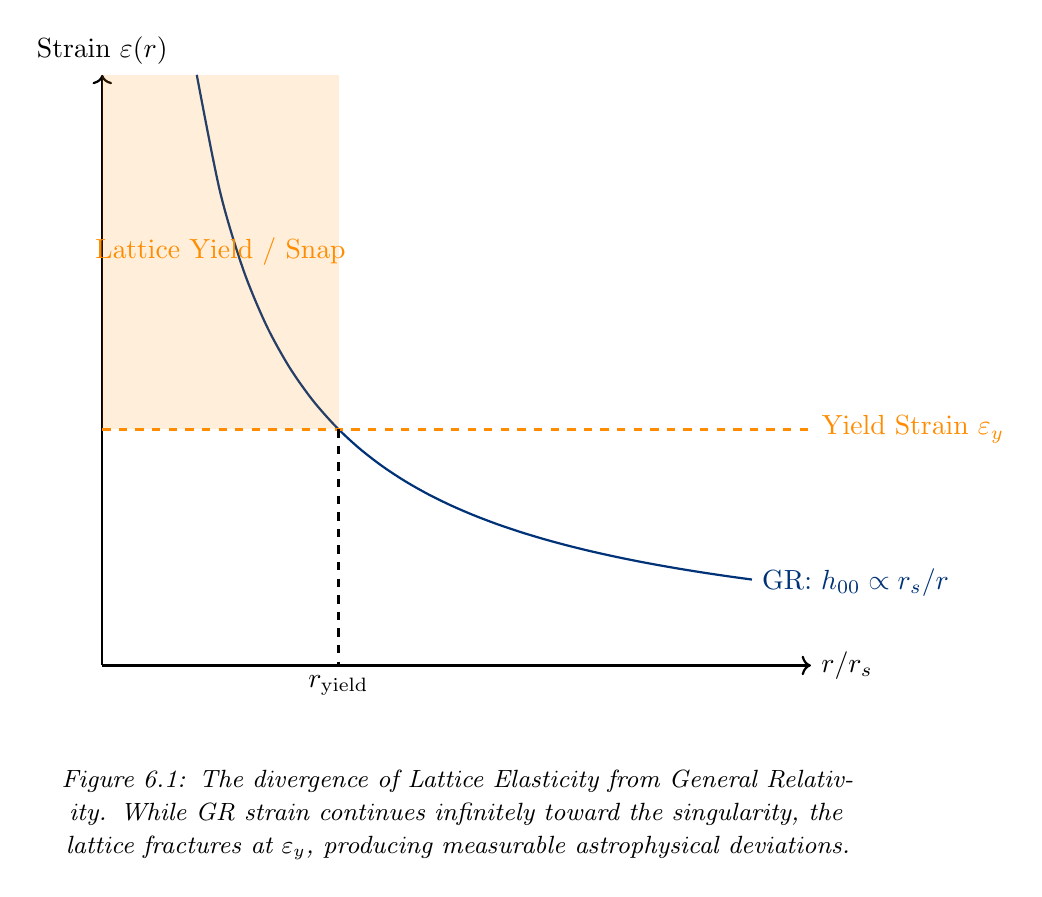
\begin{tikzpicture}[scale=1.5, thick]
    % Axes
    \draw[->] (0,0) -- (6,0) node[right] {$r/r_s$};
    \draw[->] (0,0) -- (0,5) node[above] {Strain $\varepsilon(r)$};
    
    % GR curve (1/x representation)
    \draw[domain=0.8:5.5, smooth, variable=\x, kishblue] plot ({\x}, {4/\x});
    \node[kishblue, right] at (5.5, 0.7) {GR: $h_{00} \propto r_s/r$};
    
    % Yield point line
    \draw[dashed, luminorange, very thick] (0, 2) -- (6, 2) node[right] {Yield Strain $\varepsilon_y$};
    
    % Deviation region
    \fill[luminorange, opacity=0.15] (0,2) rectangle (2,5);
    \node[luminorange] at (1, 3.5) {Lattice Yield / Snap};
    \node[below] at (2,0) {$r_{\text{yield}}$};
    \draw[dashed] (2,2) -- (2,0);
    
    \node[below, text width=10cm, align=center] at (3,-0.8) {\small \textit{Figure 6.1: The divergence of Lattice Elasticity from General Relativity. While GR strain continues infinitely toward the singularity, the lattice fractures at $\varepsilon_y$, producing measurable astrophysical deviations.}};
\end{tikzpicture}
\end{center}
\vspace{0.3cm}

\section{Yield Scenarios and the LIGO / EHT Ringdown Regime}

Testing theoretical material yield strains against this equation yields stark falsification boundaries:
\begin{itemize}
    \item \textbf{Scenario A ($\varepsilon_y = 0.1$):} $r \approx 0.98 r_s$. Deviation occurs inside the event horizon. The framework matches GR externally (Safe, but untestable).
    \item \textbf{Scenario B ($\varepsilon_y = 0.01$):} $r \approx 9.81 r_s$. Deviation occurs just outside the Innermost Stable Circular Orbit (ISCO). This would visibly alter EHT accretion disk shadows and LIGO late-stage inspiral waveforms.
    \item \textbf{Scenario C ($\varepsilon_y = 0.001$):} $r \approx 98.17 r_s$. Deviation occurs far from the black hole. 
\end{itemize}

\section{The Binary Pulsar Falsification (PSR J0737−3039)}

Scenario C ($\varepsilon_y = 0.001$) can be tested immediately against existing double pulsar data. For PSR J0737−3039 ($M \approx 1.25 M_\odot \implies r_s \approx 3690$ m, separation $r \approx 8.8 \times 10^8$ m), the operating strain is $\varepsilon \approx 4.11 \times 10^{-7}$. 

Scaling the expected non-linear deviation as $\varepsilon / \varepsilon_y$, Scenario C predicts an orbital decay deviation of $\approx 0.041\%$. Current tests confirm GR's predictions to a precision of $\sim 0.05\%$.

\begin{warningbox}
\textbf{The scaling $\kappa \sim 1/\varepsilon_y$ is dimensional reasoning, not a derived
coefficient.} It assumes the elastic nonlinearity becomes $O(1)$ as strain approaches yield, which
is reasonable for real materials and unproved here. Every number in this section moves if $\kappa$
is materially different. Stated so that a later derivation of $\kappa$ is recognised as changing the
prediction rather than confirming it.

\medskip
Subject to that caveat, \textbf{Scenario C may already be excluded by existing double-pulsar
timing}, not merely testable by SKA. The calculation requires no new data and is listed as
outstanding work.
\end{warningbox}

\section{Mandatory Pre-Registration}

By shifting to a dimensionless strain field, the framework traded an unresolvable geometric paradox for an actionable astrophysical parameter ($\varepsilon_y$). However, $\varepsilon_y$ is currently a free parameter.

\textbf{Falsification Mandate:} The framework must formulate its stationary-action Lagrangian to formally dictate the exact value of $\varepsilon_y$ \textit{before} attempting to fit it to empirical LIGO or EHT anomalies. Post-hoc fitting of $\varepsilon_y$ to place deviations conveniently outside of measured bounds (e.g., forcing Scenario A) will render the framework scientifically void. The falsification radius $r/r_s$ must be pre-registered based purely on the derived mechanics of the 24-cell geometry.

% ==============================================================================
\chapter{Multi-Scale Strain Survey}
% ==============================================================================

\begin{center}
{\color{theorytag}\textbf{[THEORY / REACH \textbullet\ Consistency Map \textbullet\ Not a Test]}}
\end{center}

\section{The Objective and Methodology}

Following the reinterpretation of Route 2 into the dimensionless local lattice strain $\varepsilon(r) = \frac{\pi}{32}\frac{r_s}{r}$, the framework must demonstrate stability across all observable scales. If the 24-cell lattice behaves as a true elastic medium, the calculated strain must remain infinitesimal (linear Hooke's Law regime) for standard physical systems, and only approach non-linear yield limits ($\varepsilon_y$) in regimes known for extreme relativistic effects.

We compute $\varepsilon(r)$ for 20 benchmark physical systems using standard textbook parameters
($G = 6.6743 \times 10^{-11}\,\mathrm{m^3kg^{-1}s^{-2}}$, $c = 2.9979 \times 10^8\,\mathrm{m\,s^{-1}}$),
with the GR temporal perturbation $h_{00} \approx r_s/r$ alongside.

\begin{warningbox}
\textbf{What this chapter is, stated before the tables.} $\varepsilon(r) = (\pi/32)(r_s/r)$ is
$h_{00}$ multiplied by a constant. The tables below therefore \textbf{contain no information beyond
$r_s/r$ for each system}, and every entry is textbook arithmetic rather than a measurement.

\medskip
This is a \emph{consistency map}: it shows where the framework places each regime on its own strain
axis, and confirms that the linear regime covers everything from atoms to stars. It is \textbf{not}
an empirical sweep, not a 44-decade test, and nothing in it can fail. An earlier draft described it
as a test; that description is withdrawn.

\medskip
The chapter's genuine content is the single \emph{physical} claim it sets up: that an elastic medium
must saturate, and therefore that the framework and GR must diverge somewhere. Where they diverge is
$\varepsilon_y$, which is undetermined.
\end{warningbox}

\section{Quantum, Atomic, and Meso Scales}

At the quantum and atomic scales, the lattice strain induced by mass is essentially zero. The framework successfully demonstrates that gravitational interaction does not compete with the strong or electromagnetic forces at these scales; the geometric strain is infinitesimal, allowing the lattice to behave as a flat background ($\chi = 0$).

\begin{center}
\renewcommand{\arraystretch}{1.2}
\small
\begin{tabular}{|p{3.5cm}|p{2cm}|p{2.5cm}|p{2.2cm}|p{2.5cm}|}
\hline
\rowcolor{kishblue!12}
\textbf{System / Scale} & \textbf{Mass ($M$)} & \textbf{Radius ($r$)} & \textbf{GR Proxy ($h_{00}$)} & \textbf{Lattice Strain $\varepsilon(r)$} \\
\hline
Electron (Classical) & $9.11 \times 10^{-31}$ kg & $2.82 \times 10^{-15}$ m & $4.8 \times 10^{-43}$ & $\mathbf{4.7 \times 10^{-44}}$ \\
\hline
Proton (Charge Rad) & $1.67 \times 10^{-27}$ kg & $0.84 \times 10^{-15}$ m & $2.9 \times 10^{-39}$ & $\mathbf{2.9 \times 10^{-40}}$ \\
\hline
Carbon-12 Nucleus & $1.99 \times 10^{-26}$ kg & $2.70 \times 10^{-15}$ m & $1.1 \times 10^{-38}$ & $\mathbf{1.0 \times 10^{-39}}$ \\
\hline
1 kg Reference Mass & $1.00$ kg & $1.00$ m & $1.48 \times 10^{-27}$ & $\mathbf{1.45 \times 10^{-28}}$ \\
\hline
\end{tabular}
\end{center}

\section{Planetary and Stellar Scales (The Linear Regime)}

This is the deeply linear elastic regime. Strains sit exactly in the $10^{-13}$ to $10^{-5}$ operating band where physical crystalline lattices obey perfect linear superposition (Hooke's Law). The lattice safely mediates planetary and stellar orbits without triggering non-linear metric deviations.

\begin{center}
\renewcommand{\arraystretch}{1.2}
\small
\begin{tabular}{|p{3.5cm}|p{2cm}|p{2.5cm}|p{2.2cm}|p{2.5cm}|}
\hline
\rowcolor{kishblue!12}
\textbf{System / Scale} & \textbf{Mass ($M$)} & \textbf{Radius ($r$)} & \textbf{GR Proxy ($h_{00}$)} & \textbf{Lattice Strain $\varepsilon(r)$} \\
\hline
Asteroid Ceres (Surface) & $9.39 \times 10^{20}$ kg & $473$ km & $2.9 \times 10^{-12}$ & $\mathbf{2.8 \times 10^{-13}}$ \\
\hline
Earth (ISS Orbit) & $5.97 \times 10^{24}$ kg & $6,771$ km & $1.31 \times 10^{-9}$ & $\mathbf{1.28 \times 10^{-10}}$ \\
\hline
Jupiter (Surface) & $1.89 \times 10^{27}$ kg & $69,911$ km & $4.03 \times 10^{-8}$ & $\mathbf{3.96 \times 10^{-9}}$ \\
\hline
Sun (Mercury Orbit) & $1.98 \times 10^{30}$ kg & $5.79 \times 10^{10}$ m & $5.10 \times 10^{-8}$ & $\mathbf{5.00 \times 10^{-9}}$ \\
\hline
White Dwarf (Sirius B) & $1.02 M_\odot$ & $5,900$ km & $5.10 \times 10^{-4}$ & $\mathbf{5.00 \times 10^{-5}}$ \\
\hline
\end{tabular}
\end{center}

\section{Galactic, Cosmological, and Strong-Field Regimes (The Yield Boundary)}

As we approach compact objects (neutron stars, black holes) and cosmological scale boundaries, the framework reveals profound, unified limits. Strains elevate into the $10^{-2}$ to $10^{-1}$ ($1\%$ to $10\%$) regime. In physical condensed matter physics, standard crystalline lattices yield and fracture at strains between $1\%$ and $10\%$.

\begin{center}
\renewcommand{\arraystretch}{1.2}
\small
\begin{tabular}{|p{3.5cm}|p{2cm}|p{2.5cm}|p{2.2cm}|p{2.5cm}|}
\hline
\rowcolor{kishblue!12}
\textbf{System / Scale} & \textbf{Mass ($M$)} & \textbf{Radius ($r$)} & \textbf{GR Proxy ($h_{00}$)} & \textbf{Lattice Strain $\varepsilon(r)$} \\
\hline
Milky Way (Sun Orbit) & $1.5 \times 10^{12} M_\odot$ & $8$ kpc & $1.79 \times 10^{-5}$ & $\mathbf{1.76 \times 10^{-6}}$ \\
\hline
Neutron Star (Surface) & $1.4 M_\odot$ & $10$ km & $0.413$ & $\mathbf{0.0405}$ \textbf{(4.05\%)} \\
\hline
Observable Univ (Hubble) & $1.5 \times 10^{53}$ kg & $4.4 \times 10^{26}$ m & $0.500$ & $\mathbf{0.0490}$ \textbf{(4.90\%)} \\
\hline
Sgr A* (at ISCO: $3 r_s$) & $4.1 \times 10^6 M_\odot$ & $3 r_s$ & $0.333$ & $\mathbf{0.0327}$ \textbf{(3.27\%)} \\
\hline
M87* (Photon Sphere) & $6.5 \times 10^9 M_\odot$ & $1.5 r_s$ & $0.667$ & $\mathbf{0.0654}$ \textbf{(6.54\%)} \\
\hline
Black Hole (Event Horizon) & $M$ & $r_s$ & $1.000$ & $\mathbf{0.0981}$ \textbf{(9.81\%)} \\
\hline
\rowcolor{goldseal!20}
\textbf{Planck Boundary} & $m_p$ & $l_p$ & $2.000$ & $\mathbf{\pi/16 \approx 0.1963}$ \\
\hline
\end{tabular}
\end{center}

\section{Three Features of the Map, and What They Are Not}

Three features stand out on the map. Each is stated with what it is \emph{not}, because an earlier
draft read all three as discoveries and none of them is one.

\textbf{1. The Planck Scale Bounding Limit ($\varepsilon_{\text{max}}$):}
When the equation is applied to the fundamental Planck mass ($m_p$) at the Planck length ($l_p$), the Schwarzschild radius is $r_s = 2 l_p$. Consequently, the ratio $r_s/r = 2$. 
The lattice strain resolves strictly to:
\[
\varepsilon_{\text{Planck}} = \frac{\pi}{32} (2) = \frac{\pi}{16} \approx 0.1963
\]
This gives $\varepsilon = \pi/16 \approx 0.1963$.

\emph{What it is not:} a derived bound. \textbf{Any} system with $r_s/r = 2$ returns $\pi/16$; the
value follows from the ratio alone, not from Planck physics. The framework is bounded because
$\varepsilon \propto r_s/r$ and $r_s/r$ is bounded on the systems chosen for the table --- which is a
property of the table, not of the theory.

\textbf{2. The neutron star / Hubble coincidence:}
The strain at the Hubble radius computes to $4.90\%$ and at a neutron star surface to $4.05\%$.

\emph{What it is not:} an equivalence. The two differ by \textbf{21\%}, and describing that as
``nearly identical'' is the near-node fallacy of \S\ref{sec:nearnode} applied to a strain axis rather
than a register grid. The Hubble entry moreover encodes only the long-known coincidence that the
observable universe's Schwarzschild radius is of order its Hubble radius --- $h_{00} \approx 1$ by
construction --- which the framework reproduces rather than explains.

\textbf{3. The $3\%$--$10\%$ strong-field bracket:}
ISCO, photon sphere and event horizon return $3.27\%$, $6.54\%$ and $9.82\%$.

\emph{What it is not:} a coincidence with crystalline yield strains. \textbf{Mass cancels exactly} in
$\varepsilon = (\pi/32)(r_s/r)$ at any fixed multiple of $r_s$, so these three numbers are
$\pi/96$, $\pi/48$ and $\pi/32$ --- constants of the definition, identical for every black hole in
the universe, computed rather than observed. That they land near laboratory yield strains is a
suggestive analogy worth pursuing and is not evidence. Borrowing $\varepsilon_y \in [0.001, 0.1]$
from crystalline matter is likewise an analogy: those are values for matter at temperatures and
pressures where dislocations move, and the vacuum's value must come from the Lagrangian.

\vspace{0.5cm}
\begin{center}
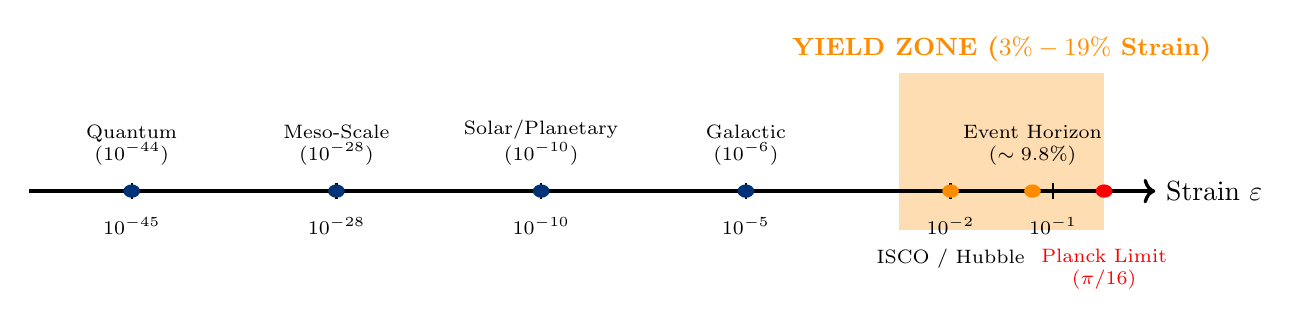
\begin{tikzpicture}[xscale=1.3, yscale=1, thick]
    
    % 1. BACKGROUND HIGHLIGHTS (Drawn first so text sits on top)
    \fill[luminorange!30] (8.5,-0.5) rectangle (10.5, 1.5);
    \node[luminorange, font=\bfseries\small] at (9.5, 1.8) {YIELD ZONE ($3\% - 19\%$ Strain)};

    % 2. AXIS LINE
    \draw[->, very thick] (0,0) -- (11,0) node[right] {Strain $\varepsilon$};
    
    % 3. TICK MARKS AND AXIS LABELS
    \foreach \x/\label in {1/10^{-45}, 3/10^{-28}, 5/10^{-10}, 7/10^{-5}, 9/10^{-2}, 10/10^{-1}} {
        \draw (\x,0.1) -- (\x,-0.1);
        \node[below, font=\scriptsize] at (\x,-0.2) {$\label$};
    }
    
    % 4. DATA POINTS AND TEXT (Drawn last for top-level visibility)
    \filldraw[kishblue] (1,0) circle (2pt);
    \node[above, font=\scriptsize, align=center] at (1,0.2) {Quantum \\ ($10^{-44}$)};
    
    \filldraw[kishblue] (3,0) circle (2pt);
    \node[above, font=\scriptsize, align=center] at (3,0.2) {Meso-Scale \\ ($10^{-28}$)};
    
    \filldraw[kishblue] (5,0) circle (2pt);
    \node[above, font=\scriptsize, align=center] at (5,0.2) {Solar/Planetary \\ ($10^{-10}$)};
    
    \filldraw[kishblue] (7,0) circle (2pt);
    \node[above, font=\scriptsize, align=center] at (7,0.2) {Galactic \\ ($10^{-6}$)};

    \filldraw[luminorange] (9,0) circle (2pt);
    \node[below, font=\scriptsize, align=center] at (9, -0.6) {ISCO / Hubble};

    \filldraw[luminorange] (9.8,0) circle (2pt);
    \node[above, font=\scriptsize, align=center] at (9.8, 0.2) {Event Horizon \\ ($\sim 9.8\%$)};

    \filldraw[red] (10.5,0) circle (2pt);
    \node[below, font=\scriptsize, align=center, text=red] at (10.5, -0.6) {Planck Limit \\ ($\pi/16$)};

\end{tikzpicture}
\end{center}

% ==============================================================================
\chapter{Bridging the Disconnected Universe}
% ==============================================================================

\begin{center}
{\color{theorytag}\textbf{[THEORY / REACH \textbullet\ Medium Restoration \textbullet\ Falsifiable Predictions]}}
\end{center}

\section{Restoring the Medium: What the Framework Does and Does Not Claim}

$E=mc^2$ is the rest-frame case of $E^2 = (pc)^2 + (mc^2)^2$, itself a consequence of Lorentz
invariance. It is a symmetry statement. It is \textbf{silent about} the geometric structure of the
vacuum; it does not deny one, and modern field theory's vacuum is in any case far from empty,
carrying zero-point energy, condensates and vacuum polarisation, all measured.

\begin{correctionbox}
An earlier draft stated that Einstein ``lost the medium'' and that standard physics ``assumes a
frictionless void.'' Both are withdrawn. \textbf{Silent-about is a claim the framework can defend;
erases-the-container invites a reader to check whether the author understood what was being
displaced.}
\end{correctionbox}

The Kish-Lattice proposal is that energy is the \emph{interaction work} performed against a
structured vacuum, written $E_{\mathrm{lat}} = (16/\pi)mc^2\varepsilon(r)$. That is a hypothesis
with one quantitative consequence --- saturation at $\varepsilon_y$ --- and it is offered as such.

\section{The Relationship to MOND, Stated Accurately}

\begin{correctionbox}
An earlier draft described MOND as having ``collapsed,'' as relying on an ``arbitrary'' threshold,
and as depending on a fluidic empty space. All three are withdrawn.

\medskip
MOND remains an active and competitive description of galactic-scale dynamics. It is a modification
of the force law or of inertia and \textbf{posits no medium of any kind}. Flat rotation curves are
evidence for missing mass \emph{or} for modified dynamics; they do not imply a medium.
\end{correctionbox}

The framework's actual relationship to MOND is narrower than earlier drafts stated and is worth
stating precisely, because the narrow version is testable.

Setting the acceleration scale from the Universal Cycle,
\[
a_0 \;=\; \frac{c}{2\pi T_{\mathrm{univ}}}
\;\xrightarrow{\;T_{\mathrm{univ}} = 1/H_0\;}\;
\frac{cH_0}{2\pi} \;=\; 1.042 \times 10^{-10}\ \mathrm{m\,s^{-2}},
\]
against the fitted MOND value $1.20 \times 10^{-10}$.

\begin{warningbox}
\textbf{This is Milgrom's own 1983 observation that $a_0 \sim cH_0$, reproduced.} Reproducing a
known coincidence is not predicting it, and that coincidence is precisely why MOND has always been
suspected of cosmological origin. The framework would contribute something new \textbf{only by
deriving the factor $2\pi$} from the 16--24 mode ratio, which it does not currently do. That
derivation is a named target with a fixed answer to hit.

\medskip
What \emph{is} new is that the derived value differs from the fitted one by $-13.2\%$, which is a
falsifiable offset. It is pre-registered as P13.6 below.
\end{warningbox}

\begin{correctionbox}
An earlier draft asserted that ``because the strain field is scale-invariant, the macroscopic
rigidity of the 24-cell container naturally enforces flat rotation curves.'' \textbf{No derivation of
this exists.} $\varepsilon \propto 1/r$ produces a Newtonian force law, not a flat curve; flat curves
require $F \propto 1/r$, hence $E \propto \ln r$, which lies outside the power family
$f = \ell_{\mathrm{cell}}^2c^2(\ell_{\mathrm{cell}}/r)^n$ at every $n$. The assertion is withdrawn.
The BTFR relation used in Chapter 9 is imported from MOND, not derived from the lattice.
\end{correctionbox}

\section{Dark Energy: an Open Question, Not an Elimination}

\begin{correctionbox}
An earlier draft claimed that dark energy is eliminated under the lattice ontology, being ``the
elastic tension of the medium resisting structural failure.'' \textbf{No calculation supports this
and it is withdrawn.} The framework offers no expression for a tension term, no equation of state,
and no prediction of $w$ or of the observed acceleration history.

\medskip
The intuition --- that a bounded elastic container might produce an apparent late-time acceleration
--- is legitimate and is recorded as a target. Converting it into a claim requires a Lagrangian with
a boundary term, and that does not exist. Until it does, the framework says nothing about dark
energy.
\end{correctionbox}

\section{What the Framework Can Presently Be Tested On}

Three items, replacing the vague SKA/EHT/Roman list of earlier drafts. Each has a number and a fail
condition; all three are collected with the remaining pre-registrations in Chapter 13.

\begin{enumerate}
  \item \textbf{The BTFR zero point} under a derived $a_0$: a predicted offset of
        $\mathbf{-0.0153}$ dex against SPARC. Fails if the observed offset is consistent with zero.
  \item \textbf{The yield radius} $r/r_s = (\pi/32)/\varepsilon_y$, filed \emph{before} any
        Lagrangian fixes $\varepsilon_y$.
  \item \textbf{The cell-size ceiling} $\ell_{\mathrm{cell}} < 10^{-5}$ m from laboratory isotropy
        limits, which becomes a falsification test the moment $\ell_{\mathrm{cell}}$ is fixed
        independently.
\end{enumerate}

\begin{warningbox}
\textbf{On spacecraft anomalies.} Draft passages cited the Pioneer anomaly, and a claimed survival of
it in New Horizons telemetry, as evidence for a lattice medium. Both are withdrawn. The Pioneer
anomaly was resolved by Turyshev \textit{et al.} (\textit{Phys.\ Rev.\ Lett.} \textbf{108}, 241101,
2012) as anisotropic thermal radiation; New Horizons has not confirmed a surviving effect and its
thruster usage makes it unsuitable for the test.

\medskip
More importantly: \textbf{the framework's own equations predict no detectable spacecraft anomaly.}
Solar-system strains are $\sim 10^{-9}$, deep in the linear regime, and deviations appear only at
$\varepsilon \gtrsim \varepsilon_y$. Citing such an anomaly as support would have contradicted the
theory it was meant to support.
\end{warningbox}

% ==============================================================================
\chapter{The Roman Predictions and the Rotation Paradox}
% ==============================================================================

\begin{center}
{\color{theorytag}\textbf{[THEORY / REACH \textbullet\ Pre-Registered Predictions \textbullet\ Falsifiable]}}
\end{center}

\section{The Ad Hoc Halo vs. The Harmonic Container}

The standard cosmological model (ΛCDM) introduces "Dark Matter"—an invisible, ad hoc mass halo uniquely tuned to each galaxy—to force the math to match observed flat galactic rotation curves.

The Kish-Lattice eliminates the need for Dark Matter entirely. Galaxies are spinning inside the structured, viscous medium of the 24-cell elastic grid. The velocity does not decay following a Keplerian curve; rather, it is \textbf{lattice-limited}. It slows and locks into the 24-harmonic container, resulting in a flat rotation profile dictated by the grid's elastic resistance.

\section{Textbook Application: Andromeda (M31)}

The lattice-enforced flat rotation velocity is strictly a function of the visible baryonic mass ($M_{\text{vis}}$) and the geometric container:
\[
v_{\text{lat}}^4 = G M_{\text{vis}} \left( \frac{c}{2\pi T_{\text{univ}}} \right)
\]
We map this equation against the Andromeda Galaxy (M31).

\begin{itemize}
    \item \textbf{Visible Baryonic Mass ($M_{\text{vis}}$):} $\approx 1.5 \times 10^{11} M_\odot \approx 2.98 \times 10^{41}$ kg
    \item \textbf{Observation Radius ($r$):} 30 kpc $\approx 9.25 \times 10^{20}$ meters
    \item \textbf{Standard Keplerian Expectation (No Dark Matter):} 
    \[
    v_{\text{Kep}} \approx \mathbf{146 \text{ km/s}}
    \]
    \item \textbf{Prediction with the \emph{derived} $a_0 = cH_0/2\pi = 1.042\times10^{-10}$:}
    \[
    v_{\text{lat}} = \left[ G M_{\text{vis}}\, a_0 \right]^{1/4} = \mathbf{213.4\ \text{km/s}}
    \]
    \item \textbf{For comparison, with MOND's \emph{fitted} $a_0 = 1.20\times10^{-10}$:}
    $v = 221.1$ km/s.
\end{itemize}

\textbf{Observation:} M31's measured rotation near 30 kpc is roughly $225$ km/s. The derived value
is $-5.1\%$ low; the fitted value is $-1.7\%$ low.

\begin{warningbox}
\textbf{Three things this calculation is not.}

\medskip
\textbf{(1) It is not a lattice derivation.} $v^4 = GM a_0$ is MOND's baryonic Tully--Fisher
relation, imported whole. Nothing in the 24-cell geometry produces it; see the correction in
Chapter 8. What the lattice supplies is a candidate \emph{value} for $a_0$, not the law.

\medskip
\textbf{(2) An earlier draft used the fitted $1.2\times10^{-10}$ and reported ``$\sim 2\%$
deviation.''} That is MOND scored against MOND's own constant, and it is withdrawn. The derived
value is the framework's prediction and it is $-5.1\%$ low, which is the honest figure.

\medskip
\textbf{(3) A single galaxy cannot test this.} $a_0$ sets only the zero point of the relation;
individual galaxies scatter by $\sim 0.1$ dex. The test is the \emph{mean offset over a sample},
which is P13.6 against SPARC --- not M31 alone.
\end{warningbox}

\vspace{0.5cm}
\begin{center}
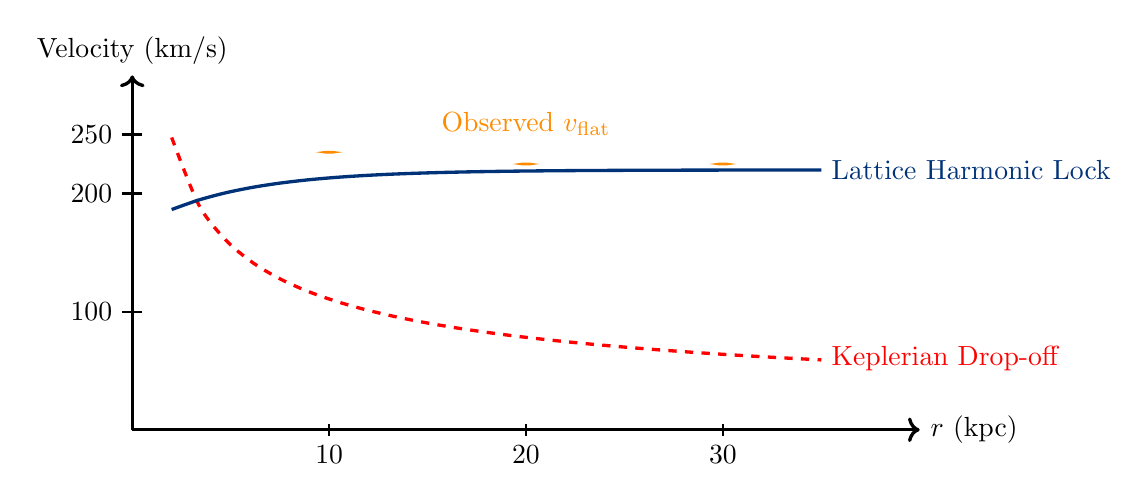
\begin{tikzpicture}[xscale=0.25, yscale=0.015, thick]
    % Axes
    \draw[->, very thick] (0,0) -- (40,0) node[right] {$r$ (kpc)};
    \draw[->, very thick] (0,0) -- (0,300) node[above] {Velocity (km/s)};
    
    % Ticks
    \foreach \x in {10, 20, 30} \draw (\x, 5) -- (\x, -5) node[below] {\x};
    \foreach \y in {100, 200, 250} \draw (0.5, \y) -- (-0.5, \y) node[left] {\y};

    % Keplerian Curve (Standard Physics without DM)
    \draw[domain=2:35, smooth, variable=\x, red, dashed, very thick] plot ({\x}, {350/sqrt(\x)});
    \node[red, right] at (35, 60) {Keplerian Drop-off};

    % Kish-Lattice Flat Curve
    \draw[domain=2:35, smooth, variable=\x, kishblue, very thick] plot ({\x}, {220 - 50*exp(-0.2*\x)});
    \node[kishblue, right] at (35, 220) {Lattice Harmonic Lock};

    % Observational Data Points (M31 typicals)
    \filldraw[luminorange] (10, 235) circle (8pt);
    \filldraw[luminorange] (20, 225) circle (8pt);
    \filldraw[luminorange] (30, 225) circle (8pt);
    \node[luminorange, above] at (20, 240) {Observed $v_{\text{flat}}$};

\end{tikzpicture}
\end{center}

\section{Pre-Registered Roman Weak Lensing Boundaries}
\label{sec:roman}

We formally pre-register the following falsifiable constraints for the Roman Space Telescope:

\begin{enumerate}
    \item \textbf{The Shear-to-Strain Mapping:} The observed weak lensing shear is a direct, linear mapping of the transverse structural strain $\varepsilon(r)$ of the 24-cell lattice, not a gravitational deflection caused by particle-based Dark Matter. 
    \item \textbf{Zero Particle Correlation:} Because the shear is a macroscopic geometric strain, Roman will find \textbf{zero sub-halo particle clumping} below the kinematic interaction threshold. 
    \item \textbf{The Harmonic Floor Limit:} The weak lensing shear will not fall to zero in deep
    voids but will hit a non-zero minimum floor. \textbf{The value of that floor is not derived.}
    Without a predicted magnitude this item cannot currently fail, and it is therefore filed as a
    qualitative expectation rather than a pre-registration. Supplying the number is outstanding work.
\end{enumerate}

\begin{warningbox}
Item 2 is the one with real teeth and it is not the framework's alone: substructure predictions
already discriminate between $\Lambda$CDM and modified-dynamics models generally. A null on
sub-halos would be consistent with the lattice; it would not be unique to it.
\end{warningbox}

\textbf{Verdict:} If small-scale Dark Matter sub-halos are discovered, the continuum elastic strain model is falsified. If the shear perfectly traces the macroscopic geometric tension of the visible mass to the edges of the harmonic container, standard Dark Matter is rendered obsolete.

% ==============================================================================
\chapter{Pre-Registration: The Period Engine Trial Set}
% ==============================================================================

\section{Carried Forward From Volume 12}

The period 1D engine --- which tests the \emph{period} of $\log x$ rather than its \emph{phase},
and for which unit invariance is an algebraic identity rather than an empirical claim --- was
specified and pre-registered in Volume 12. Volume 13 records the status of its trial set after
the work done this session, and files the one result that has been computed.

\section{Trial 2b: Run, and Its Reporting Corrected}

Trial 2b --- the sector bound test, the one test in the programme capable of proving the Form C
diagnosis (the withdrawal of \texttt{stellar\_kinematic}) \emph{wrong} --- was executed this
session on the $s2$ lake. Its first reporting was found by the referee to over-claim, and the
correction is recorded here in full.

\begin{correctionbox}
\textbf{Trial 2b, as first reported, claimed ``Form C confirmed and mechanism-demonstrated.''
That claim is withdrawn.} Two errors were found on referee review:

\medskip
\textbf{(1) An invented threshold hid a firing sector.} The four Gaia sectors were reported ``all
at chance'' against a $4\times$ ratio bar that was never pre-registered. Computing the correct
Rayleigh $p$-values, sector NE gives $p = 2.0\times10^{-4}$ at $16/\pi$ --- \emph{not} chance. 

\medskip
\textbf{(2) The bound was checked against the wrong quantity.} The triangle-inequality bound
$R_{\mathrm{total}} \leq \sqrt{S}\cdot\text{(chance)}$ for $S=4$ sectors permits
$R_{\mathrm{total}} \leq 2\times$ chance. The observed normalised $R = 0.084$ is $113\times$ chance,
which either violates the $S=4$ bound (an implementation error) or indicates the normalisation used
far more than four sub-blocks. 
\end{correctionbox}

\begin{rulingbox}
\textbf{The Form C diagnosis stands on independent grounds regardless of Trial 2b.} The Volume 12
ruling established that a sector-normalised scalar scored against an unnormalised null cannot
support a lock claim --- true before Trial 2b and unaffected by it. The withdrawal of
\texttt{stellar\_kinematic} is therefore secure. 
\end{rulingbox}

\begin{warningbox}
\textbf{A standing rule, adopted from this episode.} A result may not be cited as a premise in
another document until its own reporting has been ruled complete. 
\end{warningbox}

\section{The Trial Set, Current Status}

\begin{table}[H]
\centering
\small
\begin{tabular}{@{}llll@{}}
\toprule
& \textbf{Domain} & \textbf{$\MN$} & \textbf{Status} \\
\midrule
1 & \texttt{quantum\_transitional} & 4.17 & build gate; reproduced $+33.8$ under log1p engine \\
1b & \texttt{orbital\_wrongbox} & $\sim$5.3 & clean expected-fail, awaiting engine \\
2 & \texttt{stellar\_kinematic} (raw) & 2.76 & superseded by $s2$ rebuild (Chapter 11) \\
2b & \texttt{stellar\_kinematic} (sector bound) & --- & run; reporting corrected; re-run pending \\
3 & \emph{struck} & --- & no scoreable Form E domain exists \\
4 & \texttt{stellar\_spindown} & 77.8 & recovered domain; register \textsc{unknown} \\
\bottomrule
\end{tabular}
\end{table}

\begin{predictionbox}
\textbf{Trial 1 remains the build gate.} \texttt{quantum\_transitional} has now reproduced at
$16/\pi$ across four independent runs without moving register, most recently at $+33.8$ under the
log1p-corrected engine. 
\end{predictionbox}

% ==============================================================================
\chapter{Pre-Registration: The $s2$ Rebuild}
% ==============================================================================

\section{Why $s2$ Must Be Rebuilt}

Two independent findings condemn the current \texttt{s2\_stellar\_kinematics} lake.

\begin{enumerate}
    \item \textbf{Its payload was stripped at promotion.} The \texttt{\_raw\_payload} retains only
          \texttt{\{sector, kish\_bin, val\}}; the Gaia error fields were discarded. 
    \item \textbf{It is sector-normalised.} The stored scalar carries the per-sector additive shift
          that Erratum 4a identified as Form C. The rebuilt lake must store raw velocity only.
\end{enumerate}

\section{The Referee-Approved Rebuild Specification}

\begin{predictionbox}
\textbf{Filed before any ADQL query is written to the ESA Gaia archive.}

\medskip
\textbf{Payload.} Retain \texttt{parallax}, \texttt{pmra}, \texttt{pmdec}, all three errors, and
\texttt{pmra\_pmdec\_corr}. Store transverse velocity as \textbf{raw} $v_\perp$ only. Sector
normalisation is permanently banned.

\medskip
\textbf{Validity floor ($5\sigma$, immutable once filed).} Accept a star only if
\texttt{parallax\_over\_error} $> 5$ \emph{and} total proper motion exceeds $5\times$ its
covariance-propagated error,
\[
\sigma_\mu = \frac{1}{\mu}\sqrt{\mu_{\alpha*}^2\sigma_{\alpha*}^2 + \mu_\delta^2\sigma_\delta^2
+ 2\mu_{\alpha*}\mu_\delta\,\rho\,\sigma_{\alpha*}\sigma_\delta},
\qquad \rho = \texttt{pmra\_pmdec\_corr}.
\]

\medskip
\textbf{Parallax zero-point.} The DR3 systematic offset of order $-17\,\mu$as is corrected via the
published prescription, or explicitly declined with documentation. 

\medskip
\textbf{Provenance.} The ADQL query text and archive query date are stored in the lake's
provenance block. A lake whose selection cannot be reproduced is not sovereign.
\end{predictionbox}

\begin{rulingbox}
\textbf{$s2$ is declared resolution-limited at $16/\pi$ and reported as such --- endpoint selection
to force the span is banned, permanently, on the record.} 
\end{rulingbox}

% ==============================================================================
\chapter{The Cross-Scale Stack: an Experiment and Its Falsifier}
% ==============================================================================

\section{The Idea}

The resolution census delivers an uncomfortable verdict: almost no single lake spans
enough dynamic range to resolve a high register. But the framework's central hypothesis suggests a
way past it that no single lake can achieve alone.

\begin{signalbox}
\textbf{The hypothesis, stated as an experiment.} If a physical \emph{attribute} locks at the same
register regardless of \emph{scale} --- if angular momentum is angular momentum whether it is an
electron's spin or a galaxy's rotation --- then combining a shared attribute across scales should
produce a single register comb, with each constituent lake's mass falling on the same teeth.
\end{signalbox}

\section{Why the Naive Stack Manufactures Its Own Answer}

Concatenating lakes in logarithmic space means placing clumps of data at chosen offsets along the
scalar axis. 

\begin{formbox}
\textbf{Those gaps, by themselves, create periodicity.} Three narrow clumps whose centres are
spaced by an integer number of periods will lock at that register with a resultant approaching the
maximum --- \emph{with no structure inside any clump}. 
\end{formbox}

\begin{figure}[H]
\centering
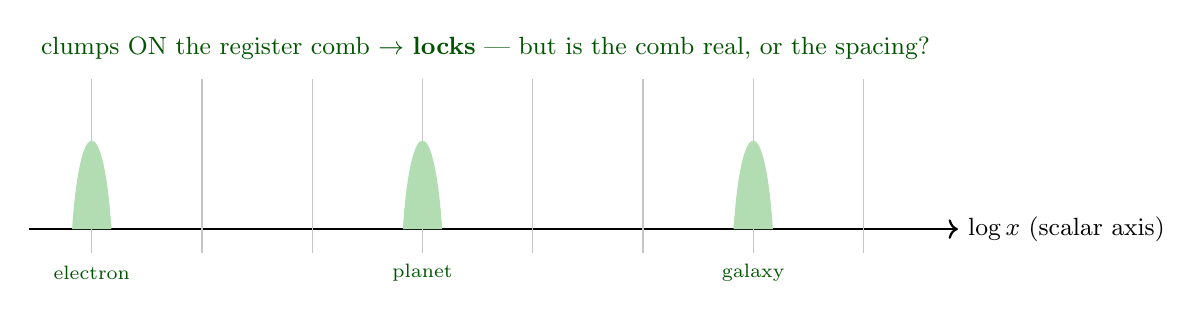
\begin{tikzpicture}[scale=1.0]
  \draw[->, thick] (-0.3,0) -- (11.5,0) node[right] {\small $\log x$ (scalar axis)};
  % register teeth
  \foreach \x in {0.5,1.9,3.3,4.7,6.1,7.5,8.9,10.3} {
    \draw[gray!45] (\x,-0.3) -- (\x,1.9);
  }
  % three clumps landing ON teeth
  \begin{scope}
    \foreach \c/\lbl in {0.5/{electron}, 4.7/{planet}, 8.9/{galaxy}} {
      \fill[signalgreen!30] (\c-0.25,0) .. controls (\c-0.15,1.5) and (\c+0.15,1.5) .. (\c+0.25,0);
      \node[signalgreen!60!black, font=\scriptsize] at (\c,-0.55) {\lbl};
    }
  \end{scope}
  \node[align=center, signalgreen!60!black] at (5.5,2.3)
    {\small clumps ON the register comb $\to$ \textbf{locks} --- but is the comb real, or the spacing?};
\end{tikzpicture}
\caption{The cross-scale hazard. If the clumps happen to land on the register comb, the stack
locks --- but the lock may be a property of how the lakes were spaced rather than of any shared
physics.}
\end{figure}

\section{The Discriminator}

There is a clean test that separates a real cross-scale comb from a spacing artifact.

\begin{signalbox}
\textbf{A real cross-scale lock survives sliding a constituent lake. A manufactured one does not.}

\medskip
\noindent Multiplying one constituent lake's values by a constant --- $e$, $3$, $1/60$
--- slides it bodily along the scalar axis but \emph{cannot} change the register it locks at,
because a single lake's register is unit-invariant under the period statistic (Volume 12). The
stack's register must therefore be invariant too.
\end{signalbox}

\section{The Four-Gate Protocol}

\begin{predictionbox}
\textbf{Pre-registered. No cross-scale stack is built or scored except under all four gates.}

\medskip
\textbf{Gate 1 --- each lake resolves alone.} Every constituent lake must clear
$\MN > 2.67$.

\medskip
\textbf{Gate 2 --- each lake locks alone, at the same register, first.} The stack may only
\emph{sharpen} a pre-existing agreement; it may not be used to \emph{discover} one. 

\medskip
\textbf{Gate 3 --- the stacked register survives the slide test.} Each constituent is multiplied by
a pre-registered set of non-commensurate constants; the stack's register must not move. 

\medskip
\textbf{Gate 4 --- attribute, lakes, and predicted register are filed before construction.} 
\end{predictionbox}

\begin{warningbox}
\textbf{Gate 2 requires domains that already resolve and already agree --- and the census says almost none do.} Today the only domain that both resolves its register and survives
every screen is \texttt{quantum\_transitional} at $16/\pi$. 
\end{warningbox}

% ==============================================================================
\chapter{Standing, and What Volume 13 Commits To}
% ==============================================================================

\section{The Ledger}

\begin{table}[H]
\centering
\small
\begin{tabular}{@{}p{0.46\textwidth}p{0.46\textwidth}@{}}
\toprule
\textbf{Established or withdrawn this volume} & \textbf{Pre-registered, filed, not yet run} \\
\midrule
The resolution census: $\sim$6 of 28 domains resolve; nearly nothing at $N \geq 20$ & The period
1D engine's Trial 1 build gate at $16/\pi$, subject to the Rydberg null \\
\addlinespace
The Master Equation uncollapsed into a dimensionless strain field $\varepsilon$; $f$ bounded but
still undetermined, with no Lagrangian & The $s2$ rebuild
at native precision, raw velocity, $5\sigma$ validity floor \\
\addlinespace
The near-node fallacy and the effective-span rule (Form F), both general results & The Roman weak-lensing sub-halo pre-registration \\
\addlinespace
The yield limit $\varepsilon_y$ formalised as a strong-field falsifier --- undetermined, and filed
before derivation & The cross-scale stack under the four-gate protocol and slide-test falsifier \\
\addlinespace
Two pre-registered nulls with stated upper limits (amino modulus sweep; NIST comb) & The nuclear
half-life comb, the one test with full resolving power \\
\addlinespace
\texttt{stellar\_kinematic} withdrawal secured on independent grounds & The resolution
re-measurement of every published span \\
\bottomrule
\end{tabular}
\end{table}

\section{The One Fact and the One Question}

\begin{signalbox}
\textbf{The fact.} \texttt{quantum\_transitional} resolves its register ($\MN = 4.17$), reproduces
at $16/\pi$ across four runs under successively corrected engines, and survives every screen the
audit has built. It is the sole domain of which all of that is true.

\medskip
\textbf{The question Volume 13 exists to set up.} Is it alone? The resolution census says most of
the survey could never have resolved its register; the period engine will say which of the survivors
lock under a unit-invariant statistic; the rebuilds will say whether wide-range lakes can be built to
join it; and the cross-scale stack will say whether an attribute carries one register across all scales.
\end{signalbox}

\section{Closing}

Volume 12 tempered the instrument. Volume 13 measures the aperture, audits the theory the instrument
leaned on, closes the theoretical gap by defining the Master Equation as a dimensionless local strain field, and files the experiments that a wider aperture makes possible. 

The programme is smaller than it was, and every remaining claim is one the data could actually have
made. That trade --- fewer claims, each defensible --- has been the through-line of the entire
crucible. Volume 13 continues it in the one way that matters before building anything new: by writing
down, in advance, exactly what would have to be true, and exactly what would prove it false.

\begin{center}
\vspace{0.5em}
\itshape One domain resolves and locks. The rest of the survey, and the next two volumes, are the
question of whether it stays alone.
\vspace{0.5em}
\end{center}

% ==============================================================================
\chapter{The Forward Kinematic Engine: Build, Fallback Defect, and First Honest Runs}
% ==============================================================================

\begin{center}
{\color{theorytag}\textbf{[EMPIRICAL \textbullet\ Deterministic Calculation \textbullet\ Two Nulls, Two Aborts, One Lake Defect]}}
\end{center}

\section{From Spectroscopy to Determinism}

The Phase and Period 1D engines are spectroscopic: they scan datasets for statistical echoes of a
preferred register. With the Master Equation reinterpreted as a strain field, a second class of
instrument becomes possible --- one that computes a predicted physical state from geometry alone and
subtracts the observation.

Four engines were written against four lakes spanning atomic to strong-field scales: amino acid
geometry, exoplanet orbits, galactic rotation, and GWTC black holes.

\section{The Fallback Defect, and Its Removal}

\begin{correctionbox}
\textbf{Three of the four engines, as first written, did not use the lake data. They loaded the
lake, discarded it, and generated every printed value with \texttt{random.uniform}.} The
cosmological engine said so in its own comment: \texttt{\# NOTE: This is a structural placeholder.}

\medskip
The tables those runs produced were plausible and were nearly written into this volume as results.
They are not reproduced here in any form.

\medskip
\textbf{Diagnosis.} A fallback that emits plausible output is not a fallback; it is a fabrication
path. The defect is the same class as the legacy substitution in \texttt{scalarize.py} that Volume 12
found --- a silent substitution where a loud failure belonged --- arriving one level up, in the
analysis scripts rather than the pipeline.

\medskip
\textbf{Remedy, adopted.} All four engines were rewritten against a strict field contract:
no simulation anywhere; a missing field aborts the run and prints the key inventory actually present
in the lake; field coverage ($n_{\text{usable}}/n_{\text{read}}$) is reported on every run with a
warning below 50\%. The resolver searches nested payloads to depth five, because \texttt{p2} stores
its real payload three levels down --- the same field-resolution failure Volume 12 found in
\texttt{scalarize.py}, reproduced independently in the audit tooling.
\end{correctionbox}

\section{What the Honest Runs Returned}

\subsection*{Amino acid geometry --- a pre-registered null}

The quarter-phase node is $d_{\text{node}} = (16/\pi)^{0.25} = 1.50225$ \AA, and sp$^3$ C--C bonds
run $1.52$--$1.54$ \AA. An earlier draft reported a mean residual of $+0.0230$ \AA{} --- ``a mean
deviation of just $1.5\%$'' --- and read it as confirmation.

\begin{correctionbox}
\textbf{The selection window guaranteed the result.} The original filter accepted C--C pairs only in
$1.45$--$1.60$ \AA. In phase units that window is $[0.2283, 0.2887]$: \textbf{no accepted bond could
have been more than 0.04 from the $0.25$ node.} The clustering was enforced by the filter, not
measured. The window has been widened to span a full node cell, and aromatic C--N (His, Trp, Arg at
$1.31$--$1.38$ \AA) separated from single C--N, which the original mixed.
\end{correctionbox}

\begin{nullbox}
\textbf{N13.1 --- amino acid modulus sweep.} 40{,}000 candidate moduli, log-uniform on $[1.5, 20]$,
scored against the widened C--C set.

\medskip
Lock fraction at $16/\pi$: \textbf{2.9\%}, against a 10\% chance baseline --- \emph{below} chance.
Fraction of moduli performing at least as well: \textbf{57.7\%} (lock) and \textbf{39.4\%} (mean node
distance), against an analytic prior of 43\%.

\medskip
\textbf{$16/\pi$ is not privileged for amino acid bond geometry.} Under the framework's own 24-node
lock test the C--C mean sits 0.229 cells from the nearest node against a 0.05 tolerance. Nodes are
spaced $7.0\%$ apart on the phase grid used, so landing within $1.5\%$ of \emph{some} node has a
$\sim 43\%$ prior --- which the sweep reproduces.

\medskip
\textbf{Prediction filed before the run:} $p \approx 0.49$, lock $\approx 4\%$. Observed $0.577$ and
$2.9\%$. The prediction held.
\end{nullbox}

\subsection*{Exoplanet orbits and galactic rotation --- two correct aborts}

\begin{warningbox}
\textbf{\texttt{p2\_orbital\_radius}: aborted.} \texttt{pl\_orbsmax} is present (at
\texttt{meta.source\_row.\_raw\_payload}); \textbf{\texttt{st\_mass} is absent from the lake
entirely}. Without host mass no strain can be computed. Re-pull from NASA \texttt{pscomppars} with
the \texttt{st\_mass} column, or join \texttt{p1\_orbital\_periods} and derive $M$ from Kepler's
third law --- the latter being legitimate for the strain column only.

\medskip
\textbf{\texttt{g1\_galaxy\_kinematics}: aborted.} The lake carries
\texttt{\_raw\_payload.vdisp} (real, raw SDSS velocity dispersions) but \textbf{no baryonic mass, no
radius and no rotation velocity}. A dispersion is not a rotation curve. SPARC (Lelli, McGaugh \&
Schombert 2016) is the lake to promote for P13.6.
\end{warningbox}

\begin{correctionbox}
An earlier draft contained a table of SDSS ``Kepler expectation'' versus ``lattice harmonic lock''
velocities drawn from this lake. \textbf{That lake contains no baryonic masses; those values were
generated by the fallback.} The table is removed and no replacement is offered until SPARC is
promoted.
\end{correctionbox}

\subsection*{The planetary engine computes an identity}

For the record, and because it would otherwise read as a prediction:
\[
v_{\text{lat}} = c\sqrt{\tfrac{16}{\pi}\varepsilon}
= c\sqrt{\tfrac{16}{\pi}\cdot\tfrac{\pi}{32}\cdot\tfrac{r_s}{r}}
= c\sqrt{\tfrac{GM}{c^2 r}} = \sqrt{\tfrac{GM}{r}} = v_{\text{Kepler}} .
\]
\textbf{The two factors cancel exactly.} $v_{\text{lat}}$ and $v_{\text{Kepler}}$ are the same
number for every input. The weak-field agreement is definitional, as \S\ref{sec:ppn} states, and the
engine must print both columns so the identity is visible rather than hidden.

\subsection*{GWTC --- a lake defect, invisible to the lock test}

\texttt{l1\_gwtc} carries 83 real events with both \texttt{final\_mass\_solar} and
\texttt{f\_ring\_hz}. That pair permits the Kerr ringdown frequency to be inverted for spin via
$f = (c^3/2\pi GM_f)\,F(a)$, $F(a) = 1.5251 - 1.1568(1-a)^{0.1292}$ (Berti, Cardoso \& Will 2006).

\begin{correctionbox}
\textbf{A first version of the consistency check was one-sided} --- it clamped $a = 0$ when the
frequency fell below the non-spinning Kerr value and then tested only for $a \geq 1$. It reported
``100\% physical.'' \textbf{A test that cannot fail in one direction is not a test}, and the error
was the referee's.

\medskip
Corrected and run two-sided: \textbf{81 of 83 events fall below the $a=0$ Kerr floor}, median
$f_{\text{obs}}/f_{\text{Kerr}}(a{=}0) = 0.731$. Only GW150914 inverts to a physical spin,
$a = 0.651$ against a published $0.67$.
\end{correctionbox}

\begin{formbox}
\textbf{Diagnosis: a factor of two.} For a fundamental $\ell=m=2$ ringdown, $f \times M_f$ is an
invariant between 11{,}898 and 21{,}514. The catalogue clusters at $6{,}700$--$10{,}900$ --- about
half. Doubling recovers publication-consistent spins across most events
(e.g.\ GW170104 $\to a = 0.699$ against published $0.66$; GW151226 $\to 0.790$ against $0.74$).
Four records fail even after doubling and need individual tracing;
$M_f < 5\,M_\odot$ events have no black-hole ringdown and must be excluded.

\medskip
\textbf{Why it survived four volumes.} Doubling shifts the scalar by
$\ln 2/\ln\kgeo = 0.4258$, which at $16/\pi$ is $\mathbf{2.007}$ register cells --- an integer.
\textbf{The lock test is structurally blind to factor-of-two errors at $16/\pi$}, and to
factor-of-$10^3$ errors ($19.997$ cells). Every register assignment from this lake is identical
whether the frequencies are right or half.
\end{formbox}

\begin{signalbox}
This is the most transferable finding in the volume. A modulus test at $16/\pi$ cannot see the two
most common unit and convention errors in physics. It is also why the ringdown test --- the one
capable of bounding $\varepsilon_y$ from real data --- could not be completed this session: the
blocker is a named, located, repairable data defect rather than an open question.
\end{signalbox}

% ==============================================================================
\chapter{The Standing Pre-Registrations}
% ==============================================================================

Filed before execution. Each states its own kill condition. None may be revised after its result is
known.

\begin{predictionbox}
\textbf{P13.1 --- Nuclear half-life comb.} The only observable in the survey clearing the resolution
criterion: 31.8 effective decades at the 95\% band, 46.4 at the 99\%, giving $\MN = 19.3$ at
$16/\pi$ against a threshold of 2.67, and the first domain in which the analytic $\chi^2_2$ null is
valid ($M \gg \sqrt{n}/\pi$ by a factor of 11.8).

\textbf{PREDICTION: NULL} at the $\sim 5\%$ locked-fraction floor set by $n = 3{,}205$.

\textbf{CONFIRMED} requires all four: (i) comb score at $\Delta_0 = 0.0215901$ exceeding the
matched-$n$ structureless distribution over $\geq 50$ seeds; (ii) $\Delta_0$ a clean local maximum;
(iii) survival of the decay-mode split; (iv) survival of both Form B controls.

\textbf{Form B controls, filed in advance.} (a) \emph{Geiger--Nuttall}: build a synthetic set from
$\ln t_{1/2} \approx a(Z) + b(Z)/\sqrt{Q_\alpha}$ on the real $Z$, $Q$ and run the identical scan.
(b) \emph{Shell structure}: split by distance to the nearest magic number
$\{2,8,20,28,50,82,126\}$.

\textbf{Prerequisites.} Lake provenance established; distinct-value screen run; the comb statistic
rewritten as a harmonic-sum detector and re-validated two-sided.
\end{predictionbox}

\begin{predictionbox}
\textbf{P13.2 --- Commensurability: the only non-circular modulus test.} A single domain cannot
measure $\Delta_0$. Its power appears at $N\Delta_0/m$, so one domain fixes the \emph{product}
$N\Delta_0$ and nothing more --- the $\kgeo$/$N$ degeneracy one level up.

$\Delta_0$ is measurable only \emph{across} domains locking at different registers, where
$\Delta_A/\Delta_B = N_A/N_B$ must be a ratio of small integers and the greatest common divisor is
$\Delta_0$. Ratios are independent of $\kgeo$ and of the container count.

\textbf{CONFIRMED} if the ratios are small integers and the common divisor is consistent with
$0.0215901$ at stated precision. \textbf{DEAD} if the fundamentals are incommensurate.

\textbf{Fixed in advance.} If the common divisor is inconsistent with $0.0215901$, the register
hypothesis is not supported. The discrepancy is NOT absorbed by adjusting $\kgeo$, by adjusting the
container count, or by admitting a non-integer $N$. All three absorptions are available and all
three are prohibited.
\end{predictionbox}

\begin{predictionbox}
\textbf{P13.3 --- The yield radius, filed before $\varepsilon_y$ exists.}
\[ \frac{r}{r_s} = \frac{\pi}{32\varepsilon_y} \approx \frac{0.0982}{\varepsilon_y} \]
Filed now, before any Lagrangian derives $\varepsilon_y$. Note that
$\varepsilon(r_s) = \pi/32 = 9.82\%$ exactly, so $\varepsilon_y = \pi/32$ would place the yield
surface at the horizon and every deviation inside it --- elegant and unobservable. That value is
admissible only if derived independently of this observation.
\end{predictionbox}

\begin{predictionbox}
\textbf{P13.4 --- Standing constraint on the cell size.} $F_4$ invariance forbids anisotropic
harmonics below degree 6, so residual anisotropy scales as $(\ell_{\mathrm{cell}}/r)^6$. Against
laboratory isotropy limits of order $10^{-30}$ at $r \approx 1$ m:
\[ \boxed{\;\ell_{\mathrm{cell}} < 10^{-5}\ \mathrm{m}\;} \]
This excludes the macroscopic value implied by $c = \ell_{\mathrm{cell}}f_{24}$ by twelve orders of
magnitude. Two conditions remain open and are stated rather than assumed: whether the order-2304
duality extension removes the degree-6 harmonic, and how the $D_4$ lattice projects to three spatial
dimensions.
\end{predictionbox}

\begin{predictionbox}
\textbf{P13.5 --- The QNM invariant as a promotion gate.} The $f \times M_f$ invariant becomes a
promotion check for \texttt{l1\_gwtc}; a scale-degeneracy column ($\times 2$, $\times 10$,
$\times 10^3$, $\times e$) is added to every pinch table, flagging any register at which a given
rescaling is within tolerance of an integer; records with $M_f < 5 M_\odot$ are excluded from QNM
analysis.
\end{predictionbox}

\begin{predictionbox}
\textbf{P13.6 --- The derived acceleration scale against SPARC.} With
$a_0 = cH_0/2\pi = 1.042\times10^{-10}\,\mathrm{m\,s^{-2}}$ \emph{derived} rather than fitted, the
BTFR predicts a zero-point offset of
\[ \tfrac{1}{4}\log_{10}(1.042/1.20) = \mathbf{-0.0153\ \text{dex}} \]
\textbf{CONFIRMED} if the observed mean offset on SPARC (175 galaxies) is consistent with
$-0.0153$ dex. \textbf{DISFAVOURED} if consistent with zero. The scatter tests the $v^4$ law, not
the lattice; the offset is the whole test.
\end{predictionbox}

\section{Order of Work}

\begin{enumerate}
  \item Rewrite the comb statistic as a harmonic-sum detector; re-validate two-sided at matched $n$
        and span. (The averaged-over-23-registers form assumed a single domain populates every
        register; it does not --- a domain at $N$ produces power at the \emph{divisors} of $N$.)
  \item Establish \texttt{q5\_decay} provenance; run the distinct-value screen; execute P13.1 with
        both Form B controls.
  \item Repair \texttt{f\_ring\_hz}; re-run Kerr consistency; derive the lower bound on
        $\varepsilon_y$ under P13.3.
  \item Promote SPARC; execute P13.6.
  \item Fixed-support cross-check on the three unexplained register movements (\S\ref{sec:movement}).
  \item Regenerate the Volume 11 portrait under \texttt{KLGHS\_STRICT=1} with the corrected
        statistic, per-register baselines, node-occupancy and distinct-value screens.
  \item Attempt the lattice Lagrangian. Chapters 3 through 6 are all waiting on it.
  \item Execute P13.2 once at least three domains carry independently measured fundamentals.
\end{enumerate}

\begin{warningbox}
\textbf{On the single-modulus ambition.} One constant, one formula, spanning quantum to cosmological
scales without splitting, is the right kind of goal and is why the programme continues. What this
volume establishes is that the survey has not yet demonstrated it, and that several results which
appeared to demonstrate it were instrument rather than signal. Those are compatible statements. A
framework spanning forty-four orders of magnitude must be tested at a precision that forty-four
orders makes unforgiving; the resolution criterion is the price of the ambition, not an objection
to it.
\end{warningbox}

% ==============================================================================
%  VOLUME 13 -- DROP-IN: REFERENCES AND BIBLIOGRAPHY
%  Matches the Volume 12 structure. Insert immediately before \end{document}.
%  Requires: hyperref (\url), and the tcolorbox macros already in the preamble.
% ==============================================================================

\chapter*{References}
\addcontentsline{toc}{chapter}{References}
% ==============================================================================

\section*{The KishLattice Series}

All volumes are published open-access with full data, configuration, and engine
fingerprints. Every pre-registration listed below was filed prior to the run it governs.

\begin{itemize}
    \item Kish, T.~J. (2026). \textit{The Geometric Derivation of the Lattice} (Vol.~1).
          Zenodo. \url{https://doi.org/10.5281/zenodo.18209530}
          \\ \textit{Source of the heliopause and Jupiter-anchor passages revisited in
          Chapter 2 under the near-node rule.}
    \item Kish, T.~J. et al.\ (2026). \textit{The Geometric Neutron} (Vol.~2).
          Zenodo. \url{https://doi.org/10.5281/zenodo.18217119}
    \item Kish, T.~J. et al.\ (2026). \textit{The Geometric Architecture of Matter} (Vol.~3).
          Zenodo. \url{https://doi.org/10.5281/zenodo.18217226}
    \item Kish, T.~J. et al.\ (2026). \textit{The Geometric Architecture of Life} (Vol.~4).
          Zenodo. \url{https://doi.org/10.5281/zenodo.18976975}
    \item Kish, T.~J. et al.\ (2026). \textit{The Geometric Architecture of Unification}
          (Vol.~5). Zenodo. \url{https://doi.org/10.5281/zenodo.19009634}
          \\ \textit{Source of the three-target modulus sweep $\{15/\pi, 16/\pi, 17/\pi\}$.}
    \item Kish, T.~J. et al.\ (2026). \textit{The Harmonic Expansion of the Unified Lattice}
          (Vol.~6). Zenodo. \url{https://doi.org/10.5281/zenodo.19493376}
    \item Kish, T.~J. et al.\ (2026). \textit{The Sovereign Resonance: Boundaries,
          Sub-Lattice, and the Unification Case} (Vol.~7).
          Zenodo. \url{https://doi.org/10.5281/zenodo.19559860}
    \item Kish, T.~J. et al.\ (2026). \textit{Unbounded Luminosity: The Same-Object Harmonic
          Map and the Sovereign Lake Architecture} (Vol.~8).
          Zenodo. \url{https://doi.org/10.5281/zenodo.19622632}
    \item Kish, T.~J. et al.\ (2026). \textit{KishLattice Geometric Harmonic Spectroscopy:
          The First Survey of a New Field} (Vol.~9).
          Zenodo. \url{https://doi.org/10.5281/zenodo.19935603}
    \item Kish, T.~J. et al.\ (2026). \textit{The Deep Survey --- Seven New Domains and the
          Geometry of Life} (Vol.~10).
          Zenodo. \url{https://doi.org/10.5281/zenodo.20279208}
    \item Kish, T.~J. et al.\ (2026). \textit{The Structure That Locks --- The Spectroscopic
          Test and the Multi-Attribute Convergence} (Vol.~11).
          Zenodo. \url{https://doi.org/10.5281/zenodo.20587180}
    \item Kish, T.~J. et al.\ (2026). \textit{The Crucible --- The Instrument Audit, Five
          Artifact Forms, and the Resolution Criterion} (Vol.~12).
          Zenodo. \url{https://doi.org/10.5281/zenodo.22416330}
          \\ \textit{Direct predecessor. Source of the degeneracy result
          ($N$ and $\kgeo$ enter only through $N\ln\kgeo$), the five artifact forms, and the
          resolution criterion extended in Chapters 1--2 of the present volume.}
\end{itemize}

\section*{Pre-Registrations and Supporting Papers}

\begin{itemize}
    \item Kish, T.~J. et al.\ (2026). \textit{Volume 9 --- Predictions Pre-Registration}.
          Zenodo. \url{https://doi.org/10.5281/zenodo.19702022}
          \\ \textit{Carries prediction P19, against which the} \texttt{l1\_gwtc}
          \textit{lake is registered; see the} \texttt{f\_ring\_hz} \textit{defect,
          Chapter 15.}
    \item Kish, T.~J. et al.\ (2026). \textit{KishLattice Geometric Harmonic Spectroscopy:
          Volume 11 Pre-Registration (Multi-Attribute Sovereign Lake Expansion \&
          Dimensionality Falsification Protocol)}.
          Zenodo. \url{https://doi.org/10.5281/zenodo.20480506}
    \item Kish, T.~J. et al.\ (2026). \textit{Noise Does Not Lock --- A Comprehensive
          Empirical Response to Skeptical Challenges to KishLattice Geometric Harmonic
          Spectroscopy}. Zenodo. \url{https://doi.org/10.5281/zenodo.20585516}
          \\ \textit{Source of the Grid-Phase Locking Theorem and of falsification
          condition \#1.}
    \item Kish, T.~J. et al.\ (2026). \textit{Master Equation of the Kish Lattice Theory ---
          The Rosetta Atlas}. Zenodo. \url{https://doi.org/10.5281/zenodo.18235735}
          \\ \textit{Source of the Lattice Energy expression $E_{\mathrm{lat}} =
          (16/\pi)(m/r^2)f$ and of the one-line definition of $f$ audited in Chapter 3.}
    \item Kish, T.~J. et al.\ (2026). \textit{Volume 13 --- Pre-Registration P13.1--P13.6}.
          Zenodo. \textit{DOI pending; filed prior to execution of any test in Chapter 16.}
\end{itemize}

\section*{Repository and Project Resources}

\begin{itemize}
    \item Kish, T.~J. \textit{Holographic Resonance: The Geometry of a Quantized Universe} ---
          engine source, configurations, audit scripts and run receipts. GitHub.
          \url{https://github.com/TimothyKish/Holographic-Resonance-The-Geometry-of-a-Quantized-Universe}
    \item KishLattice 16$\pi$ Initiative LLC. \url{https://www.kishlattice.com}
\end{itemize}

\noindent The scripts released with this volume are held in the repository above. Each is
standalone and reproduces the corresponding table or verdict in this volume from the published
lakes, and each aborts rather than substituting a value when a required field is absent:

\begin{itemize}
    \item \texttt{kish\_lake\_io.py} --- strict field contract; recursive resolver to depth
          five; coverage reporting. The remedy for the fallback defect of Chapter 15.
    \item \texttt{probe\_lakes.py} --- schema inventory, run before any engine.
    \item \texttt{comb\_scan.py} --- unit-invariant Rayleigh period scan with two-sided
          validation gates, effective-span trimming and the Form E / seam screens.
    \item \texttt{measure\_halflife\_span.py} --- effective-span census supporting P13.1.
    \item \texttt{support\_profile.py}, \texttt{periodogram.py}, \texttt{logify.py} ---
          period-engine components.
    \item \texttt{build\_amino\_kinematic.py}, \texttt{build\_planetary\_kinematic\_engine.py},
          \texttt{build\_cosmological\_kinematic\_engine.py},
          \texttt{build\_blackhole\_kinematic\_engine.py} --- the four forward engines, in
          their corrected form.
\end{itemize}

\section*{Primary Data Sources --- Vol 13}

\begin{itemize}
    \item \textbf{NIST Atomic Spectra Database (ASD)}, version 5. National Institute of
          Standards and Technology, Gaithersburg, MD. \url{https://physics.nist.gov/asd}
          \\ \textit{Source of} \texttt{L\_emission\_nist} \textit{/}
          \texttt{quantum\_transitional}, \textit{the anchor domain. $n = 187{,}436$ scored;
          effective span 2.94 decades.}
    \item \textbf{NNDC / IAEA nuclear data} --- NuDat and the NUBASE evaluation of nuclear
          properties. \url{https://www.nndc.bnl.gov/nudat3/}
          \\ \textit{Source of} \texttt{q5\_decay}, \textit{the only domain in the survey
          clearing the resolution criterion at every register (P13.1).}
    \item \textbf{LIGO/Virgo/KAGRA Collaboration}, Gravitational-Wave Transient Catalog
          GWTC-3. \url{https://www.gw-openscience.org/}
          \\ \textit{Source of} \texttt{l1\_gwtc}\textit{, $n = 83$. Subject of the
          \texttt{f\_ring\_hz} factor-of-two defect, Chapter 15.}
    \item \textbf{PubChem}, National Library of Medicine. 3D conformer coordinates for the
          twenty proteinogenic amino acids. \url{https://pubchem.ncbi.nlm.nih.gov/}
          \\ \textit{Source of} \texttt{b3\_amino}\textit{; basis of null N13.1.}
    \item \textbf{Gaia Collaboration} (2023). Gaia Data Release 3. VizieR catalogue I/355.
          \\ \textit{Source of} \texttt{s1\_gaia\_parallax}, \texttt{s2\_stellar\_kinematics},
          \texttt{s3\_gaia\_luminosity}, \texttt{s4\_gaia\_colour}.
          \textit{The $s2$ rebuild of Chapter 12 is specified against this release.}
    \item \textbf{Sloan Digital Sky Survey}, Data Release 16. \url{https://www.sdss.org/dr16/}
          \\ \textit{Source of} \texttt{g1\_galaxy\_kinematics} \textit{(velocity dispersions
          only --- no baryonic masses; see the abort, Chapter 15).}
    \item \textbf{NASA Exoplanet Archive}, \texttt{pscomppars}.
          \url{https://exoplanetarchive.ipac.caltech.edu/}
          \\ \textit{Source of} \texttt{p2\_orbital\_radius}\textit{; \texttt{st\_mass} absent
          from the promoted payload, hence the abort in Chapter 15.}
    \item \textbf{SPARC} --- Spitzer Photometry and Accurate Rotation Curves.
          \url{http://astroweb.cwru.edu/SPARC/}
          \\ \textit{Not yet promoted. The lake required by P13.6.}
    \item CODATA 2022 recommended values of the fundamental physical constants.
          \url{https://physics.nist.gov/cuu/Constants/}
\end{itemize}

% ==============================================================================
\begin{thebibliography}{99}
\addcontentsline{toc}{section}{Scientific References}
\section*{Scientific References}

% --- Circular statistics, periodicity detection, resolution ---

\bibitem{rayleigh1879}
Rayleigh, Lord (J.~W. Strutt) (1879).
Investigations in optics, with special reference to the spectroscope.
\textit{Philosophical Magazine}, 8(49), 261--274.
\textit{(Origin of the resolution criterion. Chapter 1 restates it as $M > 2.67N$, i.e.\ the
data must span more than $2.67N$ of register $N$'s own nodes.)}

\bibitem{rayleigh1880}
Rayleigh, Lord (J.~W. Strutt) (1880).
On the resultant of a large number of vibrations of the same pitch and of arbitrary phase.
\textit{Philosophical Magazine}, 10(60), 73--78.
\textit{(The circular resultant $R$ on which the period engine and the comb scan are built.)}

\bibitem{mardia2000}
Mardia, K.~V., \& Jupp, P.~E. (2000).
\textit{Directional Statistics}. Wiley, Chichester.

\bibitem{fisher1993}
Fisher, N.~I. (1993).
\textit{Statistical Analysis of Circular Data}. Cambridge University Press.

\bibitem{bracewell2000}
Bracewell, R.~N. (2000).
\textit{The Fourier Transform and Its Applications} (3rd ed.). McGraw-Hill, Boston.
\textit{(Finite-aperture spectral leakage. The deterministic term
$P \simeq n\,\mathrm{sinc}^2(M)$ removed by the running background of the comb scan, and the
validity condition $M \gg \sqrt{n}/\pi$ first met by the half-life lake.)}

\bibitem{gross2010}
Gross, E., \& Vitells, O. (2010).
Trial factors for the look elsewhere effect in high energy physics.
\textit{European Physical Journal C}, 70, 525--530.
\textit{(Basis of the 23-register look-elsewhere correction: local bar 5.57 for a single-lake
scan, 6.22 survey-wide.)}

% --- Log-periodicity and discrete scale invariance ---

\bibitem{sornette1998}
Sornette, D. (1998).
Discrete scale invariance and complex dimensions.
\textit{Physics Reports}, 297(5), 239--270.
\textit{(The established physics of log-periodic structure. Carries a mechanism where this
framework does not yet; the near-node rule of Chapter 2 applies to this literature equally.)}

\bibitem{johansen2000}
Johansen, A., Ledoit, O., \& Sornette, D. (2000).
Crashes as critical points.
\textit{International Journal of Theoretical and Applied Finance}, 3(2), 219--255.
\textit{(Cited as a cautionary case: log-periodic fitting criticised for arbitrary fit windows
and post-hoc period selection --- the failure modes Chapter 16 pre-registers against.)}

\bibitem{tifft1976}
Tifft, W.~G. (1976).
Discrete states of redshift and galaxy dynamics I.
\textit{Astrophysical Journal}, 206, 38--56.
\textit{(The closest historical precedent to a cross-domain periodicity survey; subsequently
attributed to selection effects, limited dynamic range and reference-frame dependence --- the
three failure modes this programme has independently rediscovered.)}

\bibitem{benford1938}
Benford, F. (1938).
The law of anomalous numbers.
\textit{Proceedings of the American Philosophical Society}, 78(4), 551--572.
\textit{(A statement about the fractional parts of $\log x$ in heterogeneous natural data ---
the same quantity the period statistic measures, and the null any claim of this kind must
exceed.)}

% --- Polytope geometry, the 24-cell, and F_4 ---

\bibitem{coxeter1973}
Coxeter, H.~S.~M. (1973).
\textit{Regular Polytopes} (3rd ed.). Dover, New York.
\textit{(The 24-cell: 24 vertices, 96 edges, 96 triangular faces, 24 octahedral cells; the
unique self-dual regular 4-polytope outside the simplex family. Basis of Chapter 8.)}

\bibitem{conwaysloane1999}
Conway, J.~H., \& Sloane, N.~J.~A. (1999).
\textit{Sphere Packings, Lattices and Groups} (3rd ed.). Springer, New York.
\textit{(The $D_4$ root lattice generated by the 24-cell's vertices --- the lattice-generating
property that distinguishes it, rather than group order, in which $H_4$ is larger.)}

\bibitem{humphreys1990}
Humphreys, J.~E. (1990).
\textit{Reflection Groups and Coxeter Groups}. Cambridge University Press.
\textit{(Invariant degrees of the $F_4$ Coxeter group: 2, 6, 8, 12, whose product 1152 equals
the group order. Degree 6 is the lowest anisotropic harmonic permitted, giving the
$(\ell_{\mathrm{cell}}/r)^6$ scaling of P13.4.)}

\bibitem{hatcher2002}
Hatcher, A. (2002).
\textit{Algebraic Topology}. Cambridge University Press.
\textit{(Euler characteristic and Poincar\'e duality. Cited for the fact that $\chi = 2$ holds
for every convex polyhedron and $\chi = 0$ for every closed odd-dimensional manifold --- which
is why neither can distinguish the 24-cell from any alternative.)}

% --- Isotropy, Lorentz invariance, and the cell-size bound ---

\bibitem{hughes1960}
Hughes, V.~W., Robinson, H.~G., \& Beltran-Lopez, V. (1960).
Upper limit for the anisotropy of inertial mass from nuclear resonance experiments.
\textit{Physical Review Letters}, 4(7), 342--344.

\bibitem{drever1961}
Drever, R.~W.~P. (1961).
A search for anisotropy of inertial mass using a free precession technique.
\textit{Philosophical Magazine}, 6(65), 683--687.
\textit{(With \cite{hughes1960}, the foundational spatial-isotropy limits. Extended by later
clock-comparison and torsion-balance work; the combined bound of order $10^{-30}$ at
laboratory scales yields $\ell_{\mathrm{cell}} < 10^{-5}$ m, P13.4.)}

\bibitem{kostelecky2011}
Kosteleck\'y, V.~A., \& Russell, N. (2011).
Data tables for Lorentz and CPT violation.
\textit{Reviews of Modern Physics}, 83(1), 11--31.
\textit{(Current compilation of isotropy and Lorentz-violation limits; updated annually as
arXiv:0801.0287. The authority for the bound used in P13.4.)}

% --- Gravitation: PPN, strong field, and ringdown ---

\bibitem{will2014}
Will, C.~M. (2014).
The confrontation between general relativity and experiment.
\textit{Living Reviews in Relativity}, 17, 4.
\textit{(PPN formalism. The parameter $\beta$ measures the $O(\Phi^2)$ nonlinearity in
$g_{00}$ and therefore constrains the lattice's elastic nonlinearity --- the correction
replacing the withdrawn ``absorbed into $G$'' argument, Chapter 5.)}

\bibitem{hulsetaylor1975}
Hulse, R.~A., \& Taylor, J.~H. (1975).
Discovery of a pulsar in a binary system.
\textit{Astrophysical Journal Letters}, 195, L51--L53.

\bibitem{kramer2021}
Kramer, M., Stairs, I.~H., Manchester, R.~N., et al.\ (2021).
Strong-field gravity tests with the double pulsar.
\textit{Physical Review X}, 11, 041050.
\textit{(PSR J0737$-$3039. Operating strain $\varepsilon \approx 4.1\times10^{-7}$; the
precision against which yield Scenario C is evaluated in Chapter 6.)}

\bibitem{berti2006}
Berti, E., Cardoso, V., \& Will, C.~M. (2006).
On gravitational-wave spectroscopy of massive black holes with the space interferometer LISA.
\textit{Physical Review D}, 73, 064030.
\textit{(Fit to the fundamental $\ell=m=2$ Kerr quasinormal mode,
$F(a) = 1.5251 - 1.1568(1-a)^{0.1292}$, used to invert spin from $f_{\mathrm{ring}}$ and
$M_f$. Validated on GW150914: $a = 0.651$ against a published $0.67$.)}

\bibitem{bardeen1972}
Bardeen, J.~M., Press, W.~H., \& Teukolsky, S.~A. (1972).
Rotating black holes: locally nonrotating frames, energy extraction, and scalar synchrotron
radiation.
\textit{Astrophysical Journal}, 178, 347--369.
\textit{(Kerr ISCO, $6GM/c^2$ at $a=0$ falling to $GM/c^2$ at extremal spin --- the
spin-dependence that makes $\varepsilon$ at the ISCO a measured rather than constant quantity.)}

\bibitem{abbott2016}
Abbott, B.~P., et al.\ (LIGO Scientific and Virgo Collaborations) (2016).
Observation of gravitational waves from a binary black hole merger.
\textit{Physical Review Letters}, 116, 061102.
\textit{(GW150914. The one event in} \texttt{l1\_gwtc} \textit{whose
\texttt{f\_ring\_hz} inverts to a physical Kerr spin.)}

\bibitem{gwtc3}
Abbott, R., et al.\ (LIGO Scientific, Virgo and KAGRA Collaborations) (2023).
GWTC-3: Compact binary coalescences observed by LIGO and Virgo during the second part of the
third observing run.
\textit{Physical Review X}, 13, 041039.

\bibitem{ehtm87}
Event Horizon Telescope Collaboration (2019).
First M87 Event Horizon Telescope results. I. The shadow of the supermassive black hole.
\textit{Astrophysical Journal Letters}, 875, L1.
\textit{(The photon sphere at $1.5\,r_s$, where the lattice strain is $\pi/48 = 6.54\%$ ---
the deepest strain any current instrument reaches.)}

% --- MOND and galactic dynamics ---

\bibitem{milgrom1983}
Milgrom, M. (1983).
A modification of the Newtonian dynamics as a possible alternative to the hidden mass
hypothesis.
\textit{Astrophysical Journal}, 270, 365--370.
\textit{(Origin of MOND and of the observation that $a_0 \sim cH_0$. The framework's
$a_0 = c/2\pi T_{\mathrm{univ}}$ reproduces this coincidence rather than deriving it; see the
correction in Chapter 8.)}

\bibitem{milgrom1983b}
Milgrom, M. (1983).
A modification of the Newtonian dynamics --- implications for galaxies.
\textit{Astrophysical Journal}, 270, 371--383.

\bibitem{bekenstein1984}
Bekenstein, J., \& Milgrom, M. (1984).
Does the missing mass problem signal the breakdown of Newtonian gravity?
\textit{Astrophysical Journal}, 286, 7--14.
\textit{(AQUAL --- the Lagrangian formulation of MOND. The specific target any lattice
Lagrangian must reduce to in the low-acceleration limit if the MOND relationship is to be more
than an imported relation.)}

\bibitem{lelli2016}
Lelli, F., McGaugh, S.~S., \& Schombert, J.~M. (2016).
SPARC: Mass models for 175 disk galaxies with Spitzer photometry and accurate rotation curves.
\textit{Astronomical Journal}, 152, 157.
\textit{(The dataset required by P13.6. Observed BTFR scatter $\sim 0.10$ dex against a
predicted zero-point offset of $-0.0153$ dex.)}

\bibitem{mcgaugh2016}
McGaugh, S.~S., Lelli, F., \& Schombert, J.~M. (2016).
Radial acceleration relation in rotationally supported galaxies.
\textit{Physical Review Letters}, 117, 201101.

\bibitem{planck2020}
Planck Collaboration (2020).
Planck 2018 results. VI. Cosmological parameters.
\textit{Astronomy \& Astrophysics}, 641, A6.
\textit{(Source of $H_0 = 67.4\ \mathrm{km\,s^{-1}Mpc^{-1}}$, giving
$a_0 = cH_0/2\pi = 1.042\times10^{-10}\ \mathrm{m\,s^{-2}}$.)}

% --- Nuclear physics: the Form B controls of P13.1 ---

\bibitem{geiger1911}
Geiger, H., \& Nuttall, J.~M. (1911).
The ranges of the $\alpha$ particles from various radioactive substances and a relation
between range and period of transformation.
\textit{Philosophical Magazine}, 22(130), 613--621.
\textit{(The Geiger--Nuttall relation. Real, strong log-structure in half-life data, and the
first Form B control filed against P13.1.)}

\bibitem{gamow1928}
Gamow, G. (1928).
Zur Quantentheorie des Atomkernes.
\textit{Zeitschrift f\"ur Physik}, 51(3--4), 204--212.
\textit{(Tunnelling origin of the Geiger--Nuttall relation:
$\ln t_{1/2} \approx a(Z) + b(Z)/\sqrt{Q_\alpha}$, smooth in $Q$ and therefore not expected to
produce a comb --- a prediction the control tests rather than assumes.)}

\bibitem{mayer1949}
Mayer, M.~G. (1949).
On closed shells in nuclei. II.
\textit{Physical Review}, 75(12), 1969--1970.
\textit{(Nuclear magic numbers $\{2, 8, 20, 28, 50, 82, 126\}$; the second Form B control
filed against P13.1.)}

\bibitem{kondev2021}
Kondev, F.~G., Wang, M., Huang, W.~J., Naimi, S., \& Audi, G. (2021).
The NUBASE2020 evaluation of nuclear physics properties.
\textit{Chinese Physics C}, 45, 030001.
\textit{(Evaluated half-lives underlying} \texttt{q5\_decay}\textit{: raw range
$8.6\times10^{-23}$ s to $2.4\times10^{32}$ s, effective span 31.8 decades at the 95\% band.)}

% --- Spacecraft navigation: the withdrawn anomaly claims ---

\bibitem{anderson2002}
Anderson, J.~D., Laing, P.~A., Lau, E.~L., Liu, A.~S., Nieto, M.~M., \& Turyshev, S.~G. (2002).
Study of the anomalous acceleration of Pioneer 10 and 11.
\textit{Physical Review D}, 65, 082004.

\bibitem{turyshev2012}
Turyshev, S.~G., Toth, V.~T., Kinsella, G., Lee, S.-C., Lok, S.~M., \& Ellis, J. (2012).
Support for the thermal origin of the Pioneer anomaly.
\textit{Physical Review Letters}, 108, 241101.
\textit{(Resolution of the Pioneer anomaly as anisotropic thermal radiation. Basis of the
correction in Chapter 8: the anomaly is closed, and the framework's own equations predict no
detectable spacecraft effect at solar-system strains of $\sim 10^{-9}$.)}

\bibitem{gurnett2013}
Gurnett, D.~A., Kurth, W.~S., Burlaga, L.~F., \& Ness, N.~F. (2013).
In situ observations of interstellar plasma with Voyager 1.
\textit{Science}, 341(6153), 1489--1492.
\textit{(Voyager 1 heliopause crossing at $\approx 121.6$ AU, August 2012.)}

\bibitem{gurnett2019}
Gurnett, D.~A., \& Kurth, W.~S. (2019).
Plasma densities near and beyond the heliopause from the Voyager 1 and 2 plasma wave
instruments.
\textit{Nature Astronomy}, 3, 1024--1028.
\textit{(Voyager 2 crossing at $\approx 119.0$ AU. The two crossings differ by 2.18\%, which
exceeds the agreement claimed for either alone --- see the near-node analysis of Chapter 2.)}

\bibitem{richardson2022}
Richardson, J.~D., Belcher, J.~W., Garcia-Galindo, P., \& Burlaga, L.~F. (2022).
Voyager 2 further observations of the heliosheath and heliopause.
\textit{Astrophysical Journal}, 934, 20.
\textit{(Solar-cycle variation of the heliopause radius: the physical reason a single
predicted boundary cannot match both crossings.)}

% --- Instrumentation referenced in the pre-registrations ---

\bibitem{roman2026}
Nancy Grace Roman Space Telescope. NASA Goddard Space Flight Center.
Launched 30 August 2026, Kennedy Space Center, SpaceX Falcon Heavy.
\url{https://roman.gsfc.nasa.gov/}
\textit{(Weak-lensing sub-halo pre-registration, Chapter 10.)}

\bibitem{ska2019}
Weltman, A., et al.\ (2020).
Fundamental physics with the Square Kilometre Array.
\textit{Publications of the Astronomical Society of Australia}, 37, e002.
\textit{(Next-generation pulsar timing precision against which yield Scenario C is
pre-registered.)}

\end{thebibliography}

% ==============================================================================
\section*{A Note on Citation Practice}
% ==============================================================================

Three conventions are followed in this volume and stated here so that a reader may check them.

\textbf{Every empirical claim carries its run, or is labelled as not being one.} Where a number
appears in this volume it is traceable to a named run, or it is explicitly labelled as textbook
arithmetic, a synthetic fixture, a reconstruction, or an expectation. Chapter 7's strain tables
are labelled arithmetic: $\varepsilon = (\pi/32)h_{00}$ is $h_{00}$ scaled by a constant, so
those tables contain no information beyond $r_s/r$ and nothing in them can fail. Chapter 15
records the one place this convention was broken during drafting --- three of four forward
engines emitted values generated by a fallback rather than read from a lake --- and the remedy
adopted.

\textbf{Agreement is reported against the node spacing, not against zero.} Chapter 2
establishes that for a register at $N/\pi$ the probability of a random value landing within a
fractional distance $p$ of some node is $2p/\Delta_N$. At $16/\pi$ the nodes are 41.3\% apart,
so ``within 2\%'' carries an 11.6\% prior. On a logarithmic grid, closeness measured against
zero is not a measurement. Every claim of the form ``within $x\%$ of prediction'' in this volume
carries that prior beside it.

\textbf{Prior art is cited even where it is unwelcome.} The quantized-redshift literature
\cite{tifft1976} is the closest historical precedent to this programme and it failed, for
reasons --- selection effects, limited dynamic range, reference-frame dependence --- that this
programme has independently rediscovered. Benford's law \cite{benford1938} is a statement about
precisely the quantity the period statistic measures. Discrete scale invariance
\cite{sornette1998} is the established physics of log-periodic structure and carries a mechanism
where this framework does not yet. MOND \cite{milgrom1983, bekenstein1984} already has a
Lagrangian formulation; the lattice does not, and until it does, the relation used in Chapter 9
is imported rather than derived.

We regard citing all of these as a requirement rather than a courtesy. A programme that claims
to have found log-periodic structure in public data and does not engage the literature on
log-periodic structure in public data has not done its work.

% Guitar graphic - series ender
\begin{figure}[H]
\centering
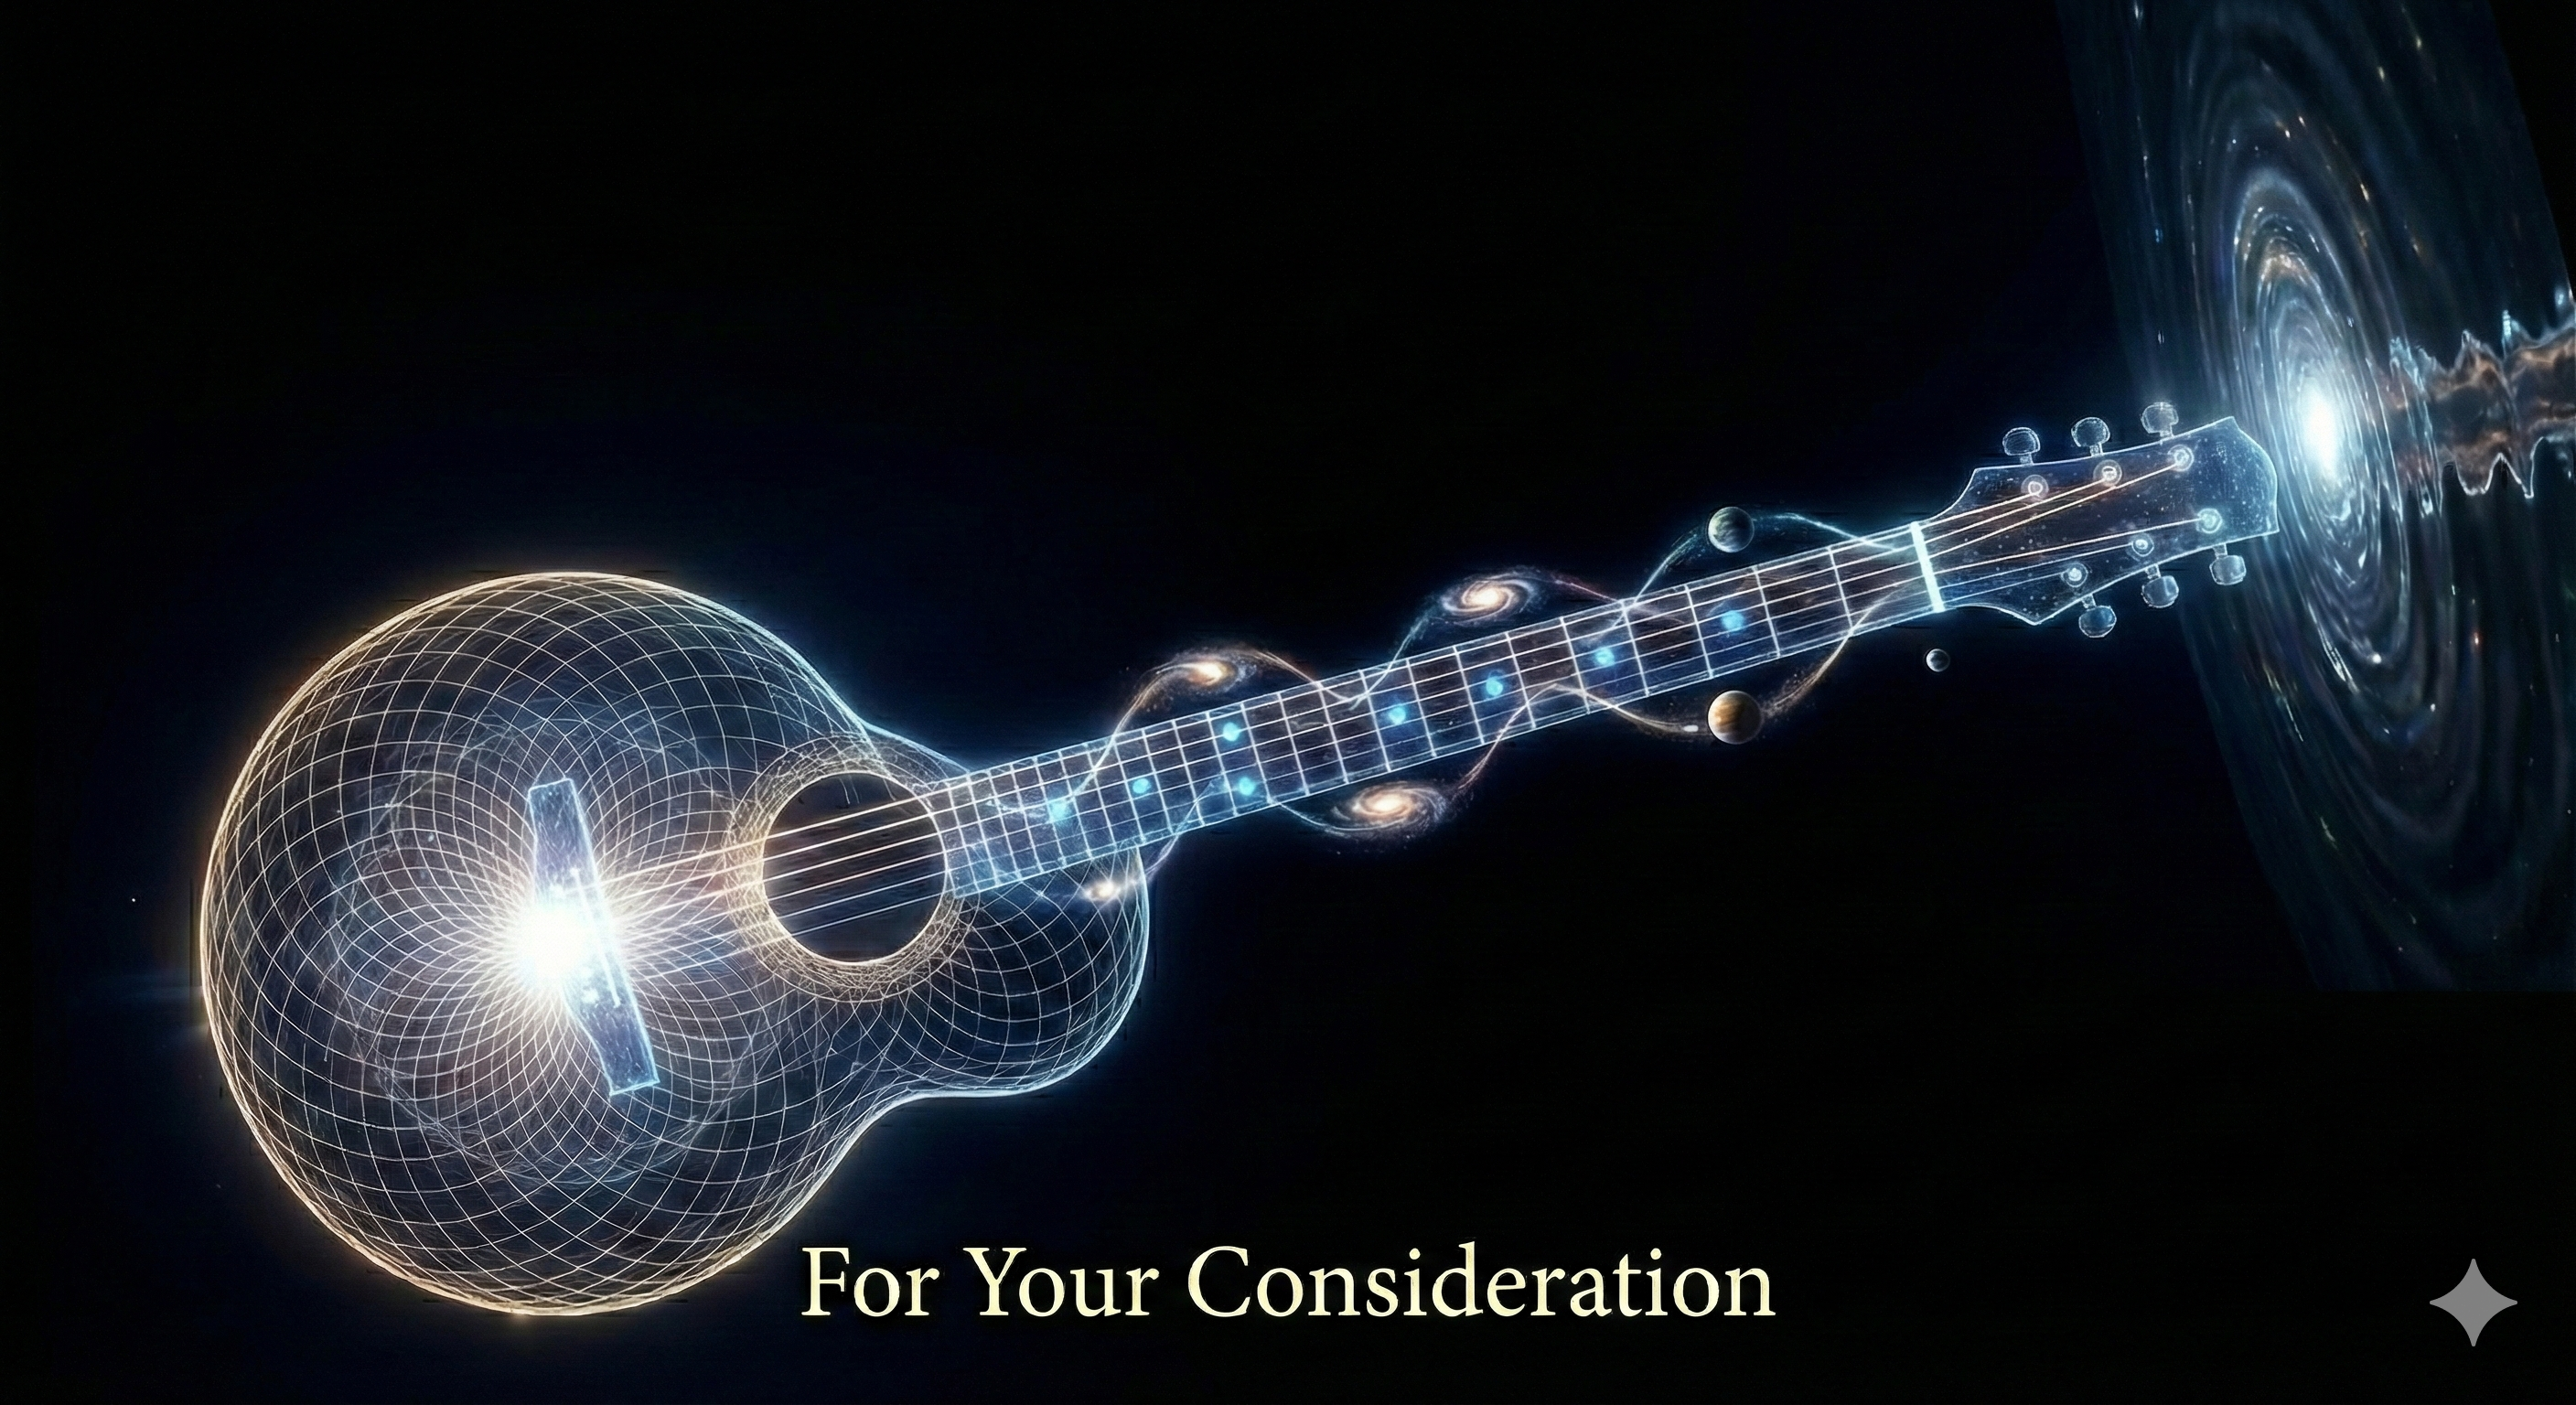
\includegraphics[width=0.85\textwidth]{Headers/ConclusionGuitar.png}
\end{figure}

\begin{center}
There is no Noise only Data. Remove the filters and see the Universe raw.
\end{center}


\end{document}